\documentclass[a4paper, 10pt]{article}
\usepackage{polski}
\usepackage[utf8]{inputenc}
\usepackage{amsmath}
\usepackage{graphicx}
\usepackage{caption}
\usepackage{subcaption}
\usepackage{geometry}
\usepackage{float}



\graphicspath{{./img/}}

\title{MGR - Raport 1}
\author{Jakub Postępski}

\begin{document}

\maketitle

\section{Wprowadzenie}
Należy skompensować siłę grawitacji w układzie stawu obrotowego sterowanego impedancyjnie. Rozwiązaniem jest określenie masy a następnie dodanie odpowiednich sił do układu w celu kompensacji siły grawitacji.

Obiektem jest układ wahadła sterowanego prawem sterowania impedancyjnego (rys. \ref{fig:2d}). Na końcu nieważkiego ramienia $r$ zawieszona jest punktowa masa $m$ której grawitację należy skompensować. Algorytm sterowania symuluje sprężynę oraz amortyzator w osi obrotu wahadła i można do niego dodać moment $u$.  Przyjmujemy że dla użytkownika dostępne są pomiary położenia $q$, prędkości $\dot{q}$, przyspieszenia $\ddot{q}$. Dodatkowo przyjmujemy, że w osi obrotu znajduje się czujnik FTS odczytujący siłę $F$ i moment siły $\tau$.

Układ z inercją $I$ możemy opisać przy pomocy równania:
\begin{equation}
\label{eq:intro}
\tau = I\ddot{q} = mr^2\ddot{q} = kq + d\dot{q} + mgr\cos{(q)} + Iu
\end{equation}

Model obiektu można opisać układem równań różniczkowych:
\label{eq:intro2}
\begin{equation}
	\begin{bmatrix}
	    \dot{q} \\
	    \ddot{q}
	\end{bmatrix}
	=
	\begin{bmatrix}
	    0 & 1 \\
	    \frac{k}{I} & \frac{d}{\tau_u}
	\end{bmatrix}
	\begin{bmatrix}
		q \\
	    \dot{q}
	\end{bmatrix}
	+
	\begin{bmatrix}
	    0 \\
	    \frac{1}{I}
	\end{bmatrix}
	(mgr\cos{(q)} + \tau_u)
\end{equation}

gdzie:
\begin{itemize}
	\item $q$ - kąt obrotu [$rad$]
	\item $k$ - sztywność
	\item $b$ - tłumienie
	\item $m$ - masa przedmiotu [$kg$]
	\item $g$ - przyspieszenie ziemskie [$\frac{m}{s^2}$]
	\item $\tau_u$ - moment dodawany w celu kompensacji grawitacji przedmiotu [$Nm$]
\end{itemize}

Układ możemy więc zapisać w standardowej postaci
\begin{equation}
\dot{q} = \textbf{A}q + \textbf{B}u(t)
\end{equation}
gdzie:
\begin{equation}
\mathbf{A} = 	\begin{bmatrix}
	    0 & 1 \\
	    \frac{k}{I} & \frac{d}{I}
	\end{bmatrix}
\end{equation}
oraz:
\begin{equation}
\mathbf{B} = \begin{bmatrix}
	    0 \\
	    1
	\end{bmatrix}
\end{equation}

Siła działająca na układ jest sumą siły grawitacji i siły odśrodkowej układu.
Siłę grawitacji możemy opisać wzorem:
\begin{equation}
F_g = mg
\end{equation}
a siłę odśrodkową odpowiednio w osi $X$ oraz $Y$ wzorami:
\begin{equation}
F_{ox} =  \cos{(q)}m\dot{q}^2 r
\end{equation}
\begin{equation}
F_{oy} =  \sin{(q)}m\dot{q}^2 r
\end{equation}


Dlatego odczyty czujnika w dwóch osiach możemy opisać wzorami:

\begin{equation}
F_x = F_{ox} = \cos{(q)}m\dot{q}^2 r
\end{equation}

\begin{equation}
\label{eq:fy}
F_y = F_g + F_{oy} = mg + \sin{(q)}m\dot{q}^2 r
\end{equation}


\section{Dyskretyzacja układu}
Po zdyskretyzowaniu metodami ZOH z okresem próbkowania $T$ otrzymujemy układ:
\begin{equation}
q(t+1) = \mathbf{A_d}q(t) + \mathbf{B}_du(t)
\label{eq:dyskretny}
\end{equation}

Dyskretyzację odczytów FTS  oraz innych równań można przeprowadzić korzystając z dyskretyzacji metodą Eulera ($\dot{q} \approx \frac{q(t)-q(t-1)}{T}$).

\begin{equation}
F_{dx}(t) = \cos{(q)}m(\frac{q(t)-q(t-1)}{T})^2 r
\end{equation}
\begin{equation}
F_{dy}(t) = mg + \sin{(q)}m(\frac{q(t)-q(t-1)}{T})^2 r
\end{equation}

oraz z równania \ref{eq:intro}
\begin{equation}
\tau(t) = kq(t) + d\frac{q(t)-q(t-1)}{T} + Iu + \cos(q)mg
\end{equation}

Podobnie można dyskretyzować inne równania i w dalszej części raportu zastosowanie metody nie będzie pokazywane wprost. We wszystkich symulacjach przedstawionych dalej użyto dyskretnych wersji przedstawionych równań.

\section{Estymacja nieznanych parametrów}
W celu skompensowania grawitacji zawieszonej masy należy poznać parametry opisujące tę masę. Uznano że do opisu wystarczą typowe i powszechnie używane zmienne. W opisywanym układzie nie są znane takie wielkości jak inercja, masa oraz środek ciężkości.

Przy założeniu, że masa jest punktowa wiemy że inercję tej masy opisuje zależność
\begin{equation}
I = mr^2
\end{equation}
W trakcie opisu metod estymacji parametrów starano się w miarę możliwości nie korzystać z tej zależności. Dzięki takiemu podejściu w przyszłości będzie można wykorzystać znalezione metody w celu estymacji mas niepunktowych o nierównomiernym rozkładzie.

Posiadając estymację promienia $r$ i wykorzystując pozycję $q$ jesteśmy w wstanie określić pozycję zawieszonej w układzie masy i jej środek ciężkości.


\subsection{Estymacja masy przy wykorzystaniu FTS}
\label{sec:ftsods}
Korzystając z równania \ref{eq:fy} można opisać siły działające na czujnik w osi $Y$ w chwili $i$ jako:
\begin{equation}
F_{yi}  = m(g + \dot{q_i}^2r\sin{(q_i)})
\end{equation}

Zakładając błędy odczytu $e$ dostajemy próbkę postaci:
\begin{equation}
\hat{F_{yi}}+e_i  = F_{yi}
\end{equation}

Posiadając $n$ próbek możemy więc sformułować zadanie optymalizacji nieliniowej z parametrami $m$ oraz $r$ takie że:
\begin{equation}
\begin{aligned}
& \underset{m, r}{\text{min}}
& & \sum_{i = 1}^{n} || e_i || = \sum_{i = 1}^{n} || \hat{F_{yi}} - F_{yi} || \\
& \text{przy ograniczeniach}
& & F_{yi} = m(g + \dot{q_i}^2r\sin{(q_i)}), \; i = 1, \ldots, n.
\end{aligned}
\end{equation}

Analogicznie można rozwiązać problem estymacji inercji $I$ wykorzystując równanie \ref{eq:intro} i sformułować zadanie optymalizacji:
\begin{equation}
\begin{aligned}
& \underset{I}{\text{min}}
& & \sum_{i = 1}^{n} || e_i || = \sum_{i = 1}^{n} || \hat{\tau_{i}} - \tau_{i} || \\
& \text{przy ograniczeniach}
& & \tau_{i} = I\ddot{q_i}^2, \; i = 1, \ldots, n.
\end{aligned}
\end{equation}

\subsection{Estymacja inercji z macierzy układu}
\label{sec:pos}
Ponieważ macierz $\mathbf{B}$ ma tylko jeden wyraz różny od zera $\mathbf{B_d}$ jest uzyskiwana w prosty sposób i można przyjąć że:
\begin{equation}
\mathbf{B_d} \approx \mathbf{B}T
\end{equation}
Przekształcając równanie \ref{eq:dyskretny} i stosując pseudoinwersję macierzy otrzymujemy równanie macierzowe:
\begin{equation}
\mathbf{A_d} = (X(t+1) - \mathbf{B}_du(t))(X(t))^{pinv}
\label{eq:pinv}
\end{equation}
przy założeniu $n$ ostatnich próbek zmiennych stanów układu
\begin{equation}
X(t) = 	\begin{bmatrix}
x(t) & x(t-1)  & ... & x(t-n)
\end{bmatrix}
\label{eq:xk}
\end{equation}

Po obliczeniu estymacji $\mathbf{A_d}$ metodą ZOH wyliczamy estymację macierzy $\mathbf{A}$ otrzymując macierz
\begin{equation}
\mathbf{\hat{A}} = 	\begin{bmatrix}
a_{11} & a_{12}\\
a_{21} & a_{22}
\end{bmatrix}
\end{equation}
Po przyrównaniu jej do macierzy $\mathbf{A}$ możemy wyliczyć inercję z równań:
\begin{equation}
\hat{I_1} = \frac{-k}{a_{21}}
\end{equation}
\begin{equation}
\hat{I_2} = \frac{-b}{a_{22}}
\end{equation}

i ostatecznie przyjąć estymację:
\begin{equation}
\hat{I} = \frac{\hat{I_1}+\hat{I_2}}{2}
\end{equation}


Metoda nie pozwala na uzyskanie wszystkich parametrów lecz w przypadku braku czujnika FTS lub uzyskania z niego zaszumionych odczytów można uzyskać tą metodą zadowalające wyniki.

\section{Kompensacja grawitacji}
Kompensacja polega na dodaniu do układu momentu siły który przeciwdziała sile grawitacji masy. Z równania \ref{eq:intro2} wynika postać sterowania $u$ kompensującego siłę grawitacji. Ponieważ zależy nam na tym aby pozbyć się członu związanego z macierzą $\mathbf{B}$
\begin{equation}
	\begin{bmatrix}
	0 \\
	1
	\end{bmatrix}
	(\frac{mgr\cos{(q)}}{I} + u) = 	\begin{bmatrix}
	0 \\
	0
	\end{bmatrix}
\end{equation}
możemy przyjąć sterowanie:
\begin{equation}
u_s(t) = -\frac{mgr\cos{(q(t))}}{I}
\end{equation}
Masę $m$, promień $r$ oraz inercję $I$ uzyskujemy z estymacji przedstawionych w sekcji \ref{sec:ftsods}.


Algorytm kompensacji nie powinien wprowadzać gwałtownych zmian w prezentowanym układzie więc sterowanie kompensujące wpływ grawitacji jest załączany stopniowo. W celu uzyskania takiego efektu sterowanie jest mnożone przez odpowiednią funkcję trapezową. Dla czasu $t_p$ początku załączania algorytmu i $t_k$ końca załączania mamy:
\begin{equation}
u(t) = \min{(\frac{\max{( t - t_p, 0)}}{t_k-t_p}, 1)}u_s(t)
\end{equation}


\section{Realizacja praktyczna}
Wszystkie symulacje układu można wykonać wykorzystując równania dyskretne (np. rys. \ref{fig:system}). W celu emulacji zakłóceń w każdym kroku symulacji zmiennych stanu układu dodawany jest szum biały. Zadane problemy optymalizacji nieliniowej rozwiązywano algorytmem Levenberga–Marquardta. Algorytm służącym do obliczania pseudoinwersji był algorytm Moora-Penrose'a.

Estymacja parametru promienia $r$ z czujnika FTS zaczyna być obarczona błędem jeśli załączony zostaje algorytm kompensacji grawitacji. Z uwagi na ten fakt zdecydowano się na podział działania programu na dwie fazy. W pierwszej poznawane są parametry modelu. W drugiej zapamiętane wcześniej promień służy do wyliczania momentu potrzebnego do kompensacji grawitacji (rys. \ref{fig:mrozenie}). Możemy przyjąć takie założenie, gdyż w rzeczywistości jeśli umieścimy masę w układzie nie będzie ona znacznie zmieniać swojego promienia. Estymacja masy i inercji w obu metodach jest nieczuła na opisany problem. Powoduje to oscylacje widoczne w układzie. O tym jak szybko układ z załączoną kompensacją grawitacji się ustabilizuje decydują wartości zmiennych stanu układu w momencie rozpoczęcia kompensacji.\\



\section{Podsumowanie}

Przedstawiony algorytm pozwala sprawnie kompensować grawitację masy układu.

Od algorytmu kompensacji siły oczekujemy, że układ powinien się zachowywać tak jakby nie była na nim zawieszona żadna masa (rys. \ref{fig:mala}). Kompensacja (rys. \ref{fig:kompensacja}) nie uwzględnia energii układu która powstała przed załączeniem kompensacji, lecz człon amortyzatora pozwala na szybkie wytracenie tej energii. Zmodyfikowany algorytm dwufazowy pozwala w szybki i skuteczny sposób radzić sobie z przedstawionym problemem jednak jego wadą pozostaje opóźnienie potrzebne na to aby zidentyfikować parametry masy umieszczonej w układzie.





\begin{figure}[H]
	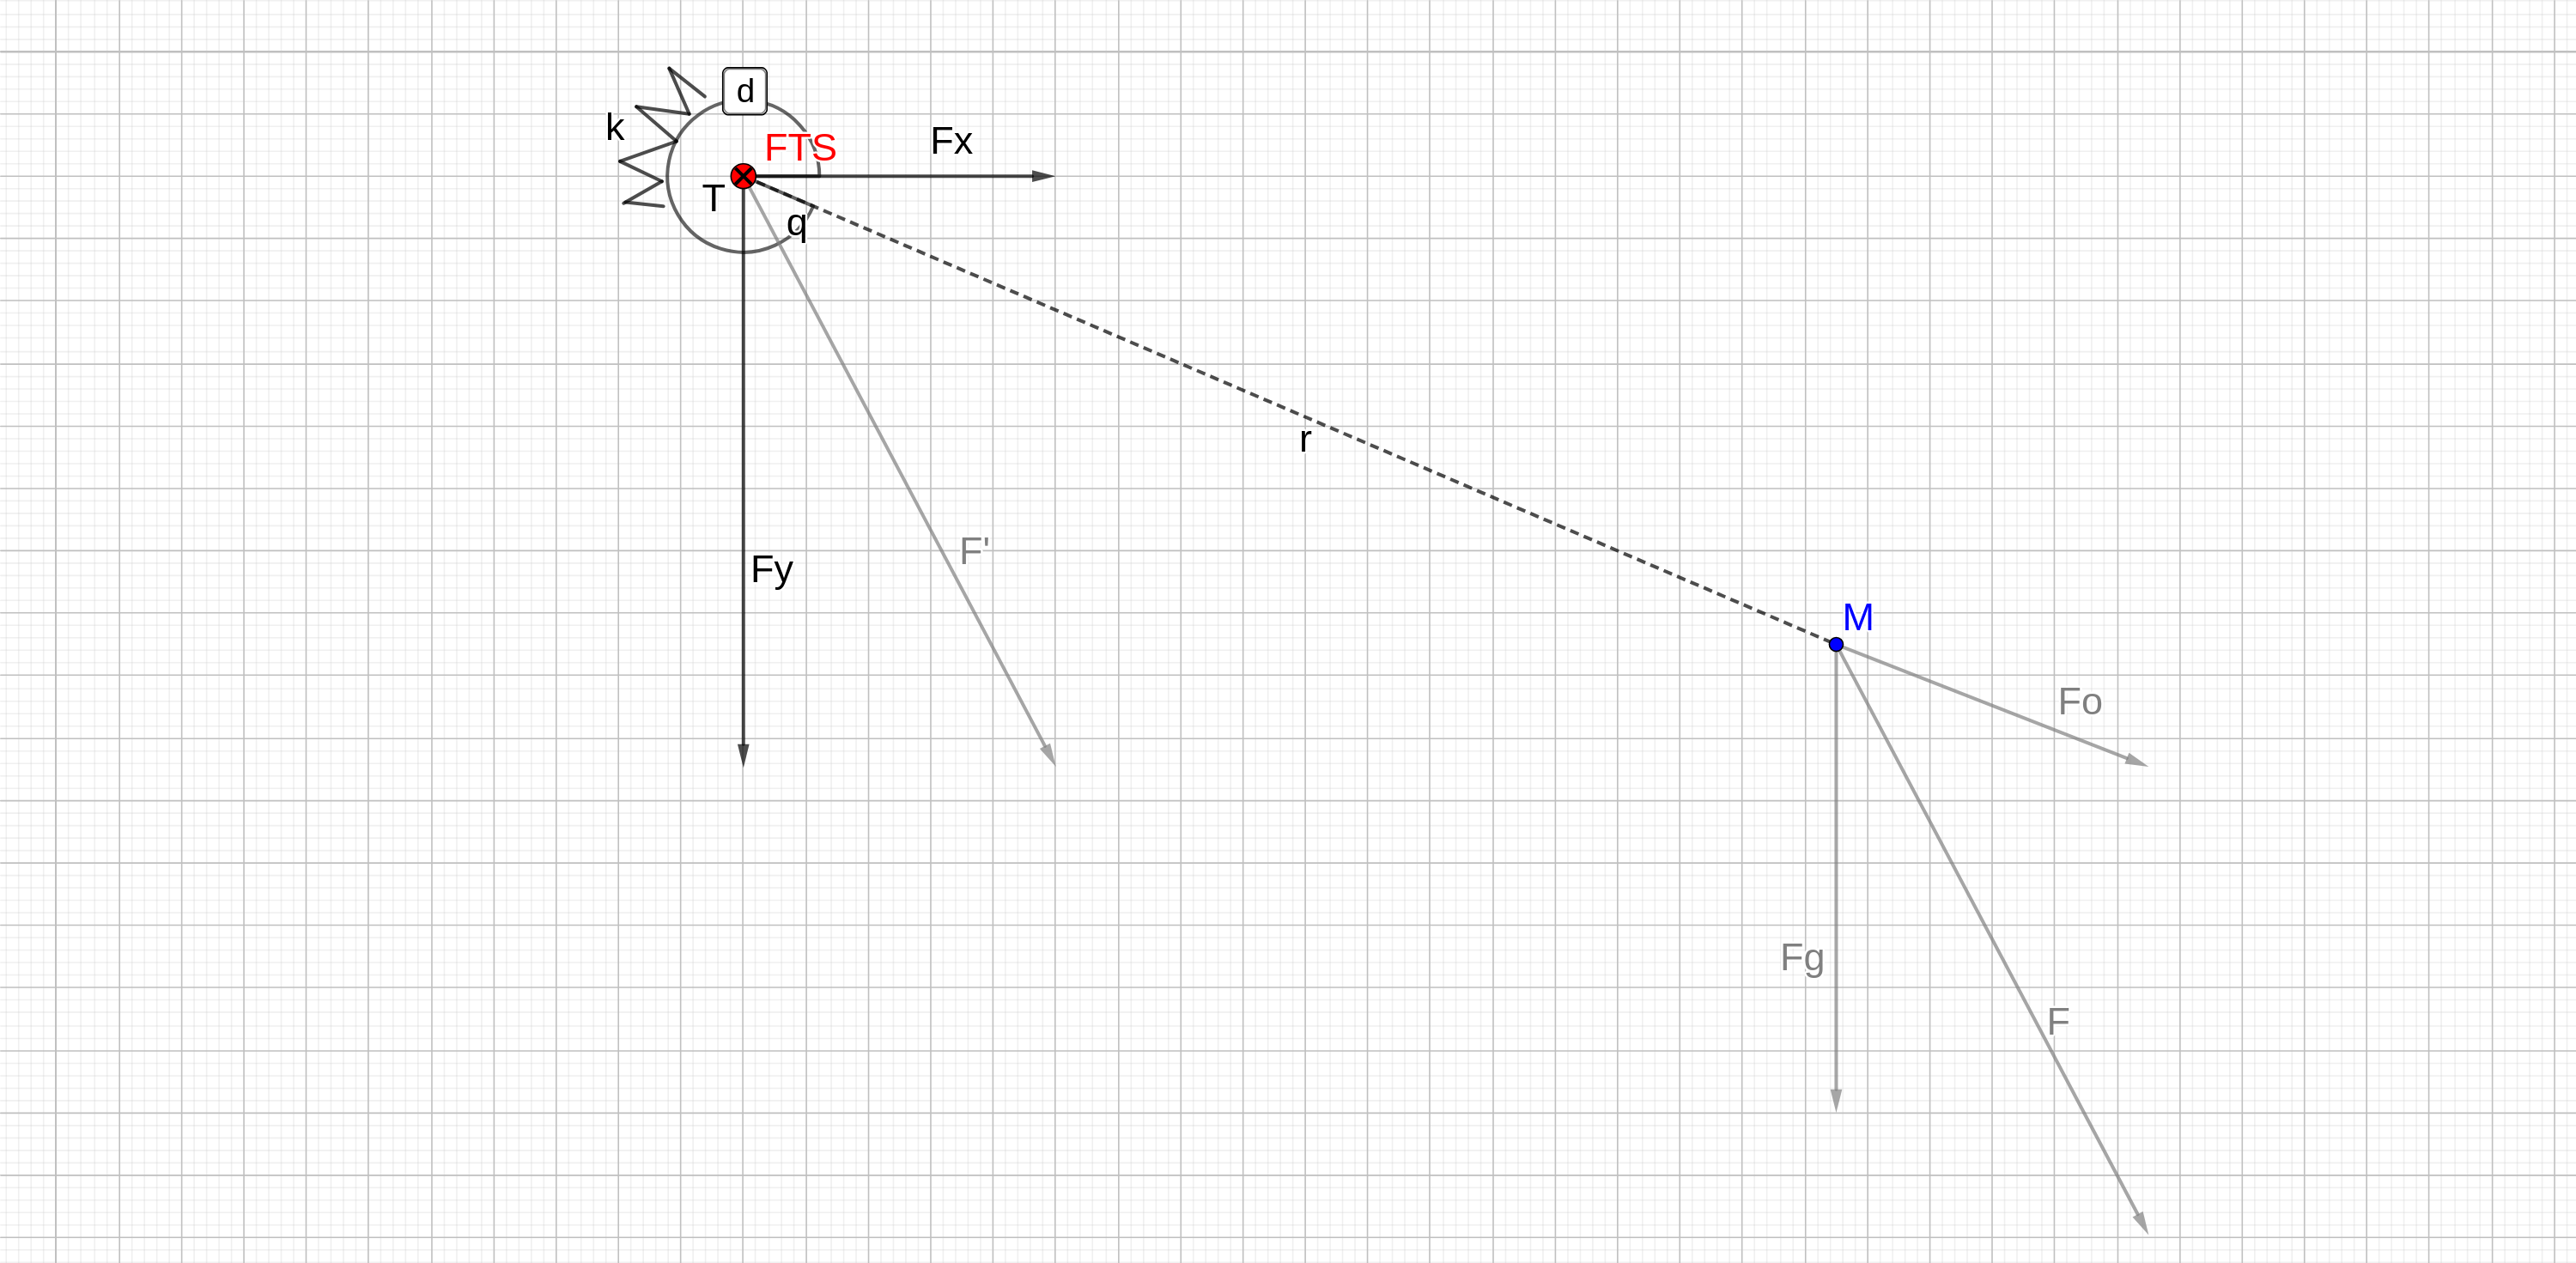
\includegraphics[width=0.99\linewidth]{2d}
	\centering
	\caption{Schemat badanego układu. Kolorem niebieskim zaznaczono masę $m$ zawieszoną na ramieniu $r$. Kolorem czerwonym zaznaczono punkt mocowania ramienie i umiejscowienia czujnika FTS. Kolorem czarnym pokazano siły odczytywane z czujnika sił, moment siły $\tau$, pozycję $q$ sprężynę $k$ oraz amortyzator $d$. Kolorem szarym zaznaczono rzeczywiste siły układu.}
	\label{fig:2d}
\end{figure}


\begin{figure}
	\centering
	\begin{subfigure}{.5\textwidth}
		\centering
		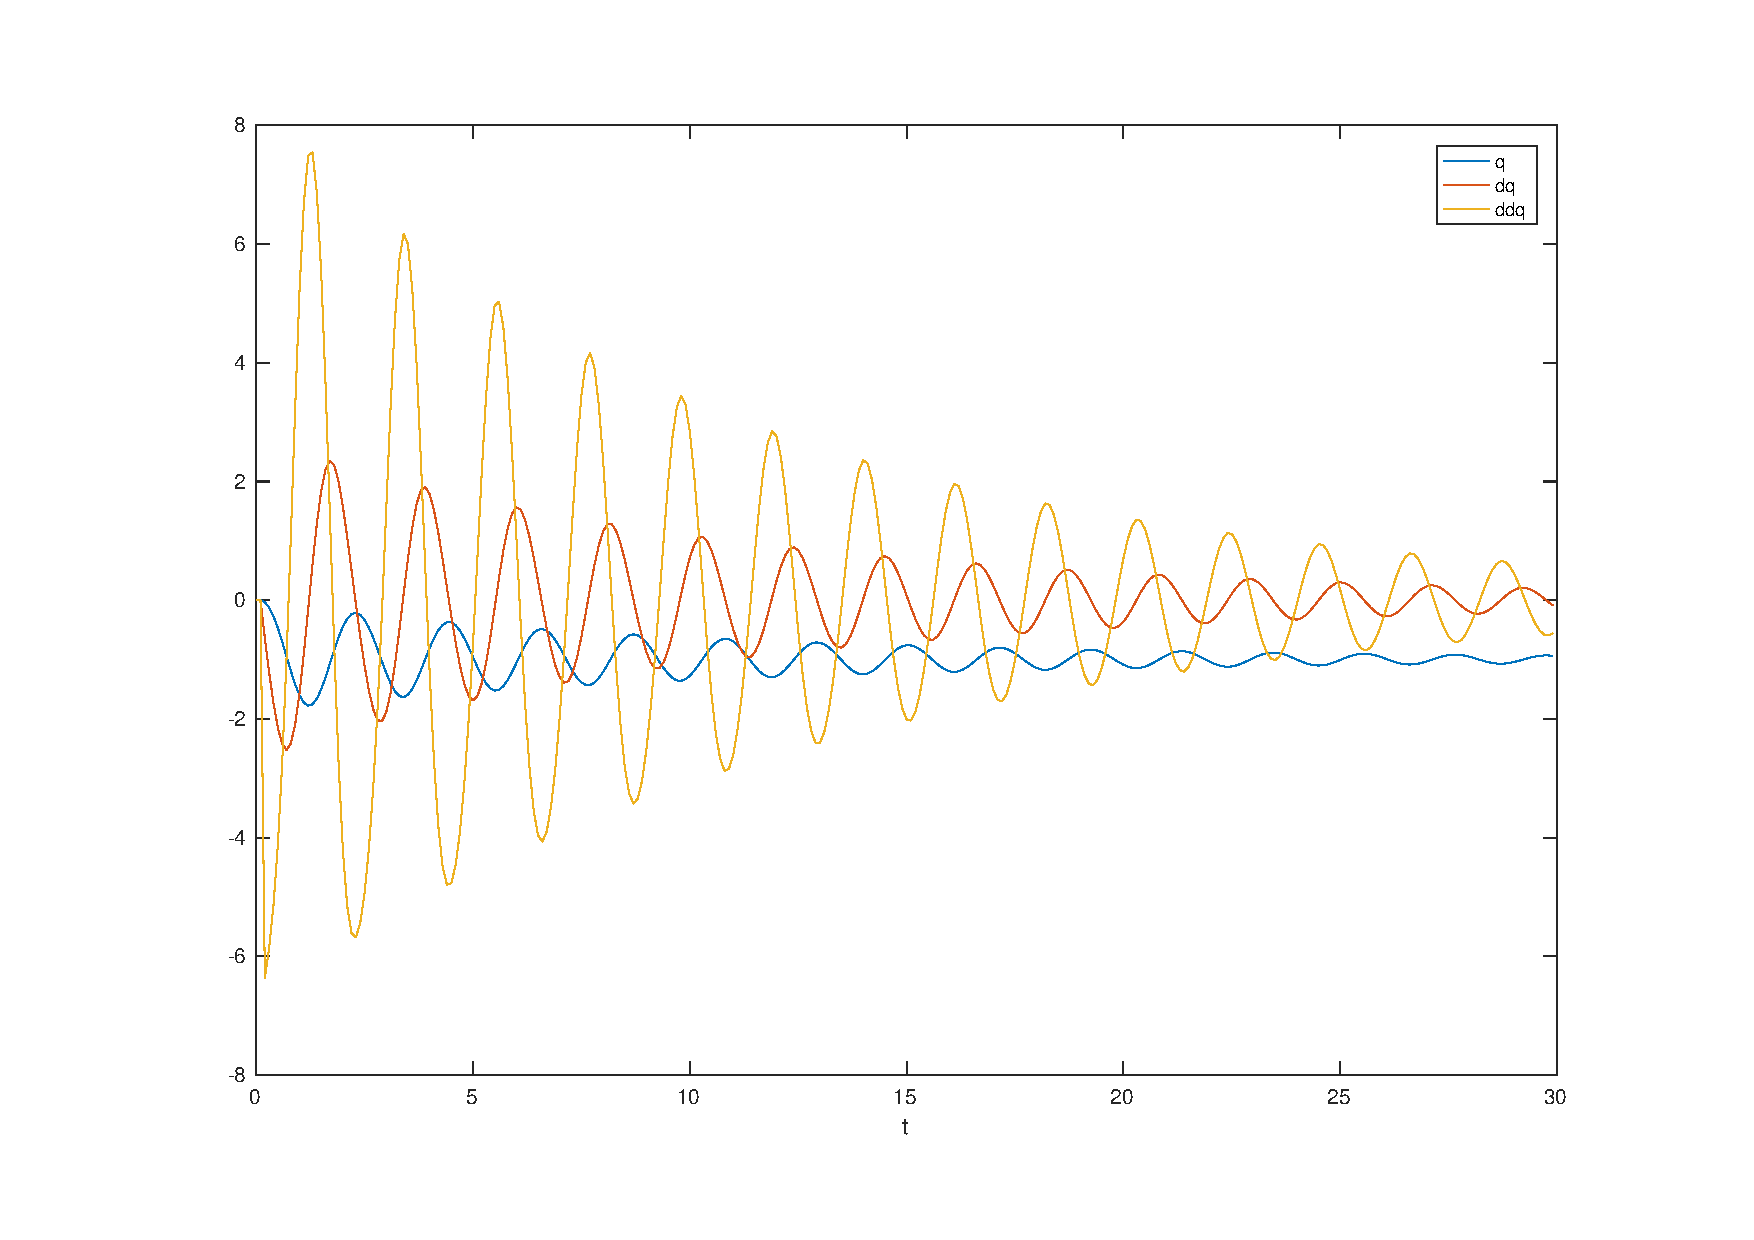
\includegraphics[width=\linewidth]{test_p}
		\caption{Stan układu. Pozycja (q), prędkość (dq) i przyspieszenie (ddq).}
		\label{fig:system_p}
	\end{subfigure}%
	\begin{subfigure}{.5\textwidth}
		\centering
		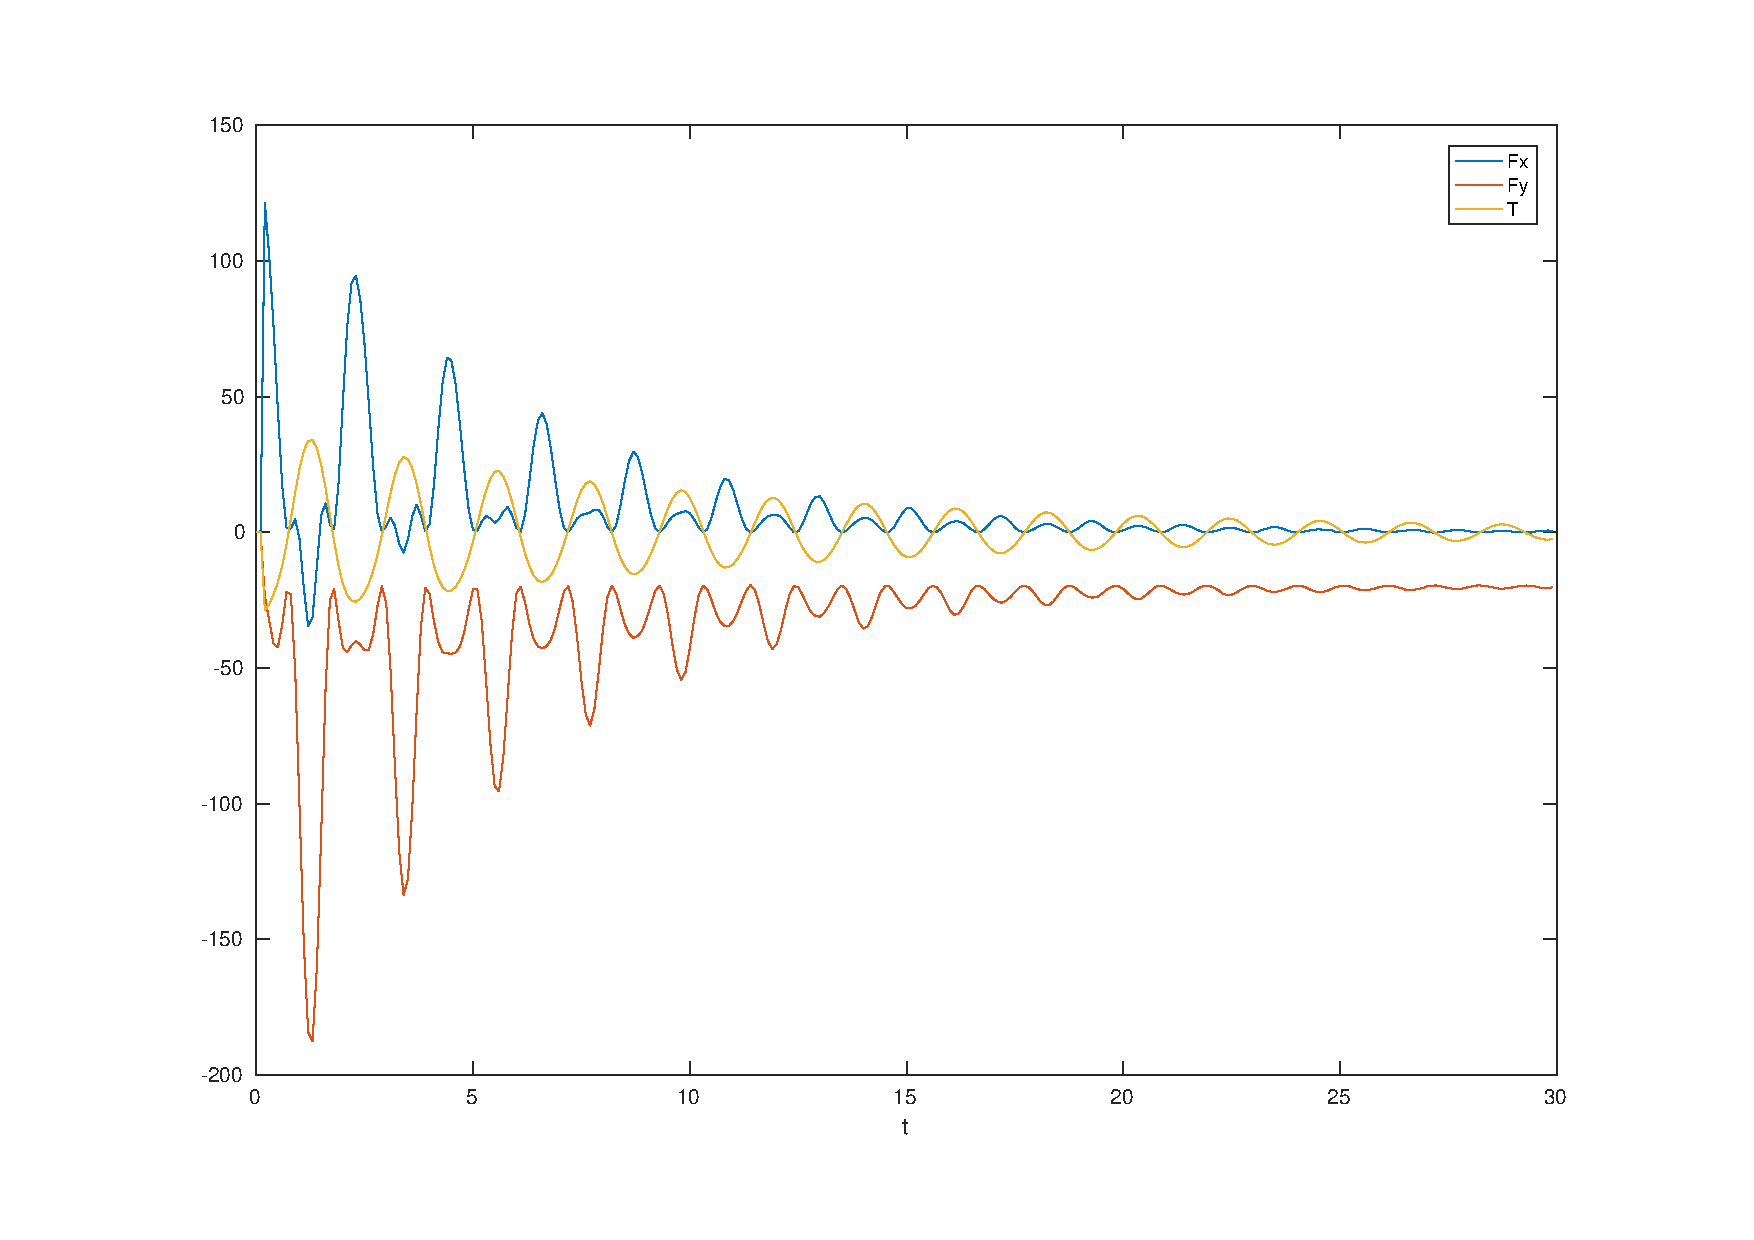
\includegraphics[width=\linewidth]{test_s}
		\caption{Odczyty czujnika FTS. Siła odczytana w osi $OX$ (Fx), w osi $OY$ (Fy) oraz moment siły (T).}
		\label{fig:system_s}
	\end{subfigure}
	\begin{subfigure}{.5\textwidth}
		\centering
		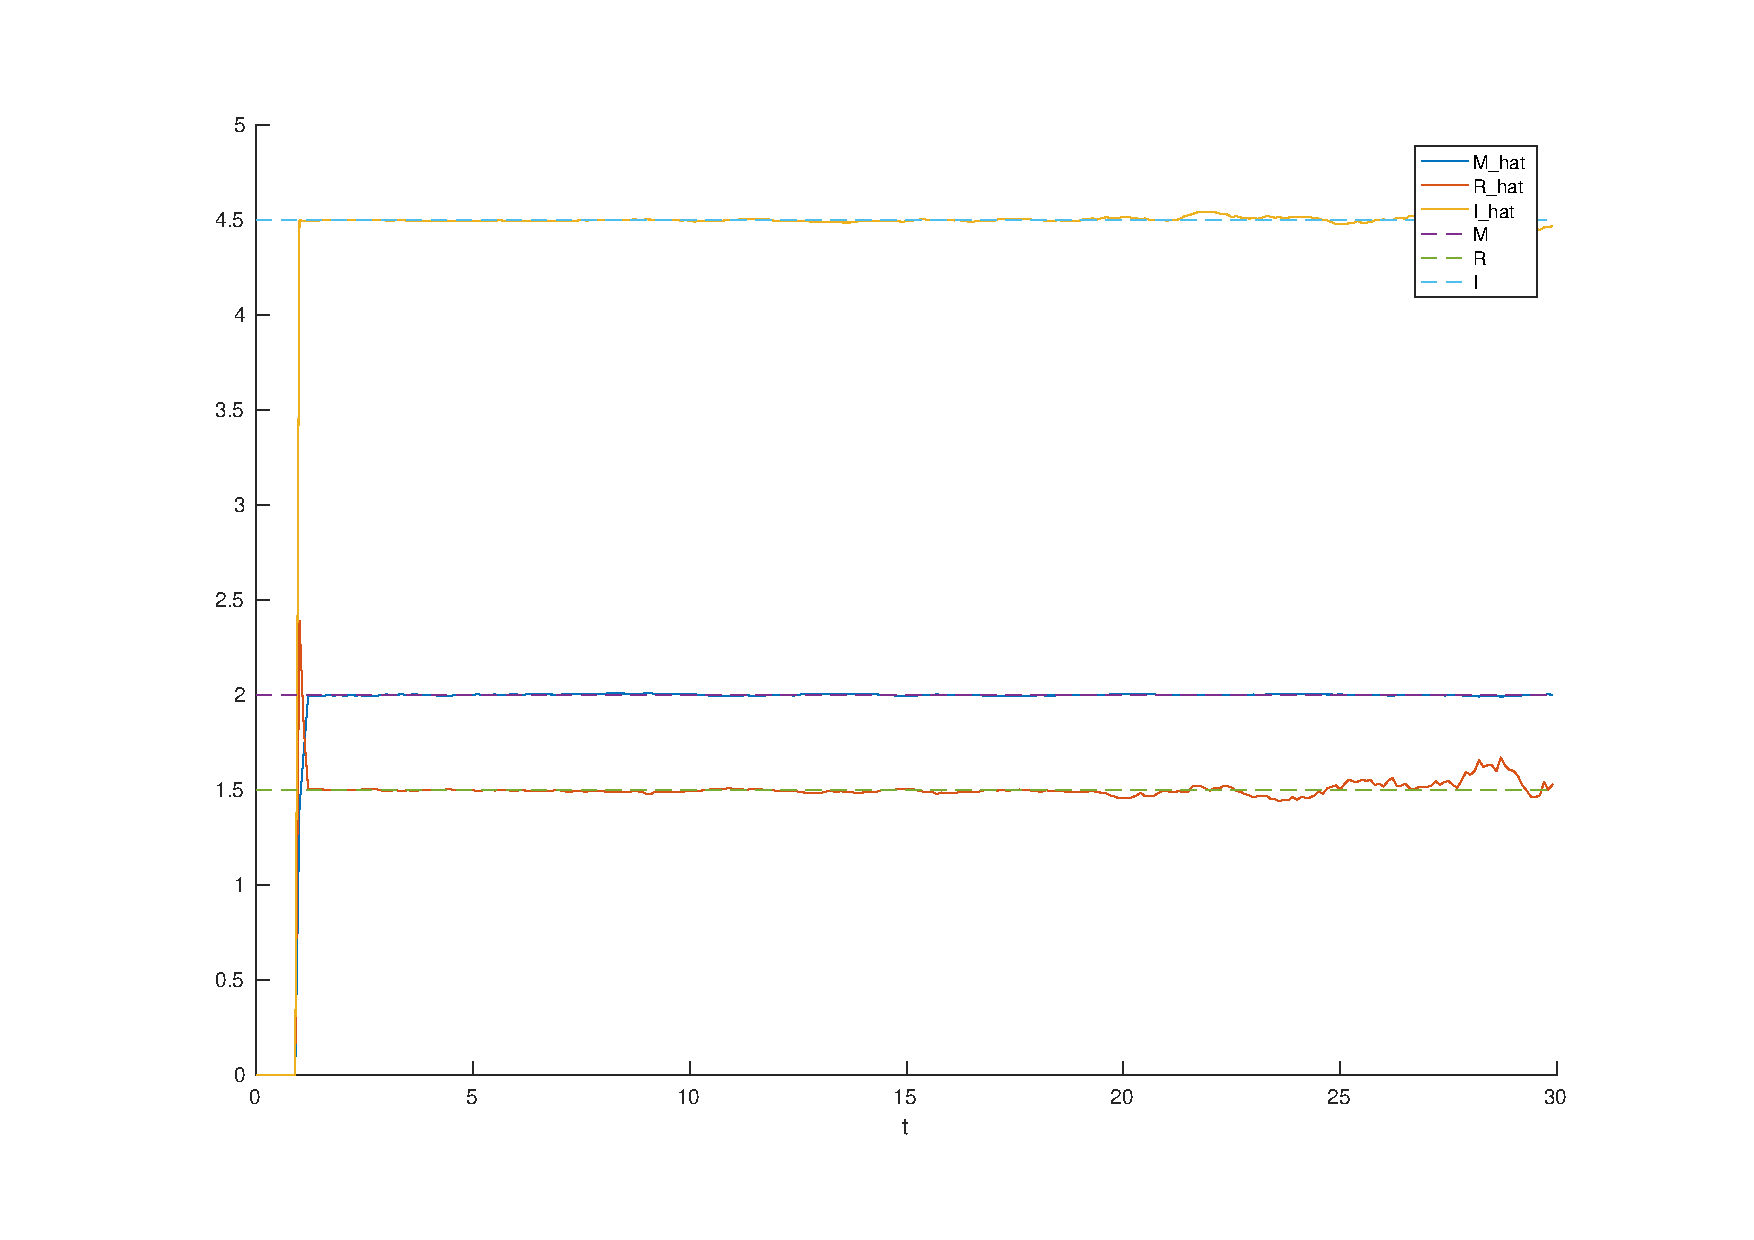
\includegraphics[width=\linewidth]{test_c}
		\caption{Estymacja parametrów z czujnika sił. Masa (M\_hat), promień (R\_hat) i inercja (I\_hat). Przerywane linie pokazują rzeczywiste wartości parametrów.}
		\label{fig:system_c}
	\end{subfigure}%
	\begin{subfigure}{.5\textwidth}
		\centering
		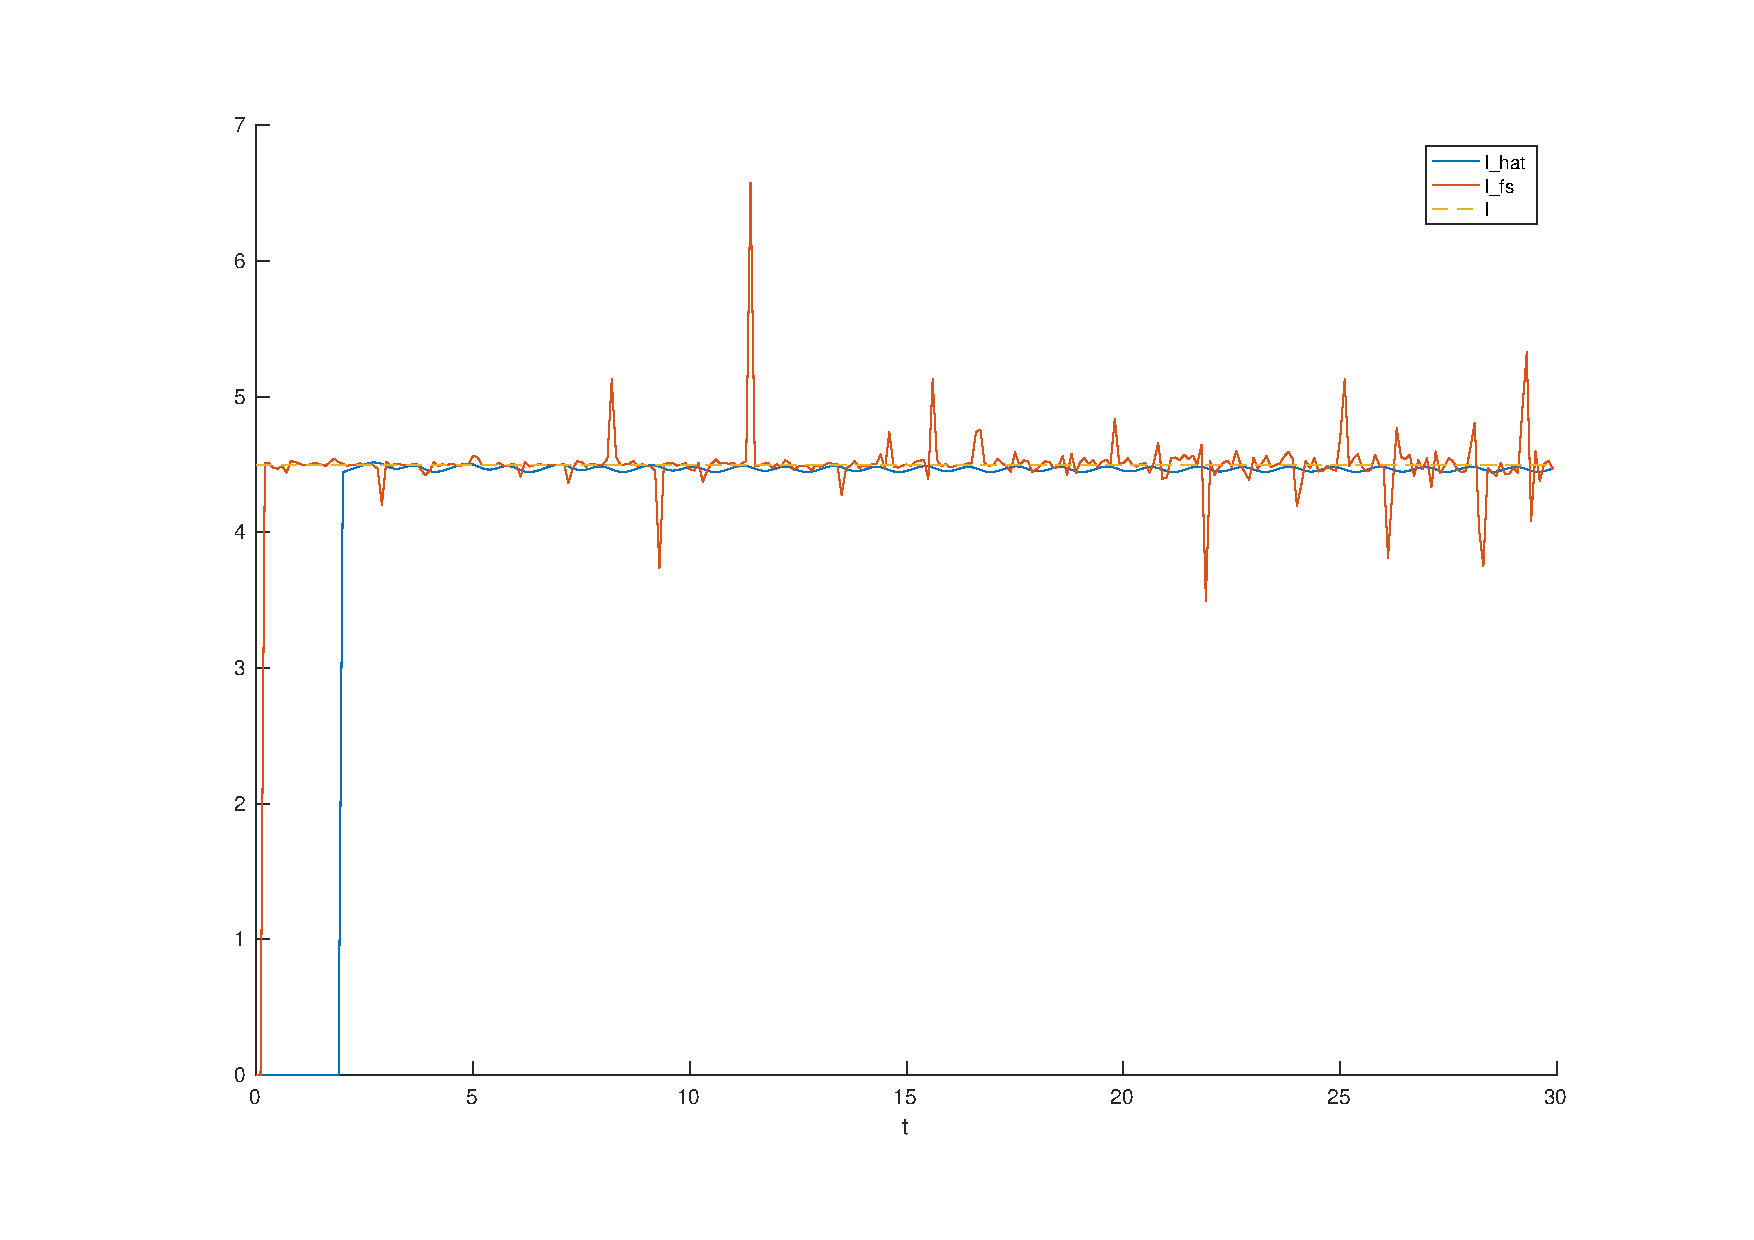
\includegraphics[width=\linewidth]{test_r}
		\caption{Estymacja inercji (I\_hat) z równań stanu. Przerywana linia pokazuje rzeczywiste wartości parametru.}
		\label{fig:system_r}
	\end{subfigure}

	\begin{subfigure}{.5\textwidth}
		\centering
		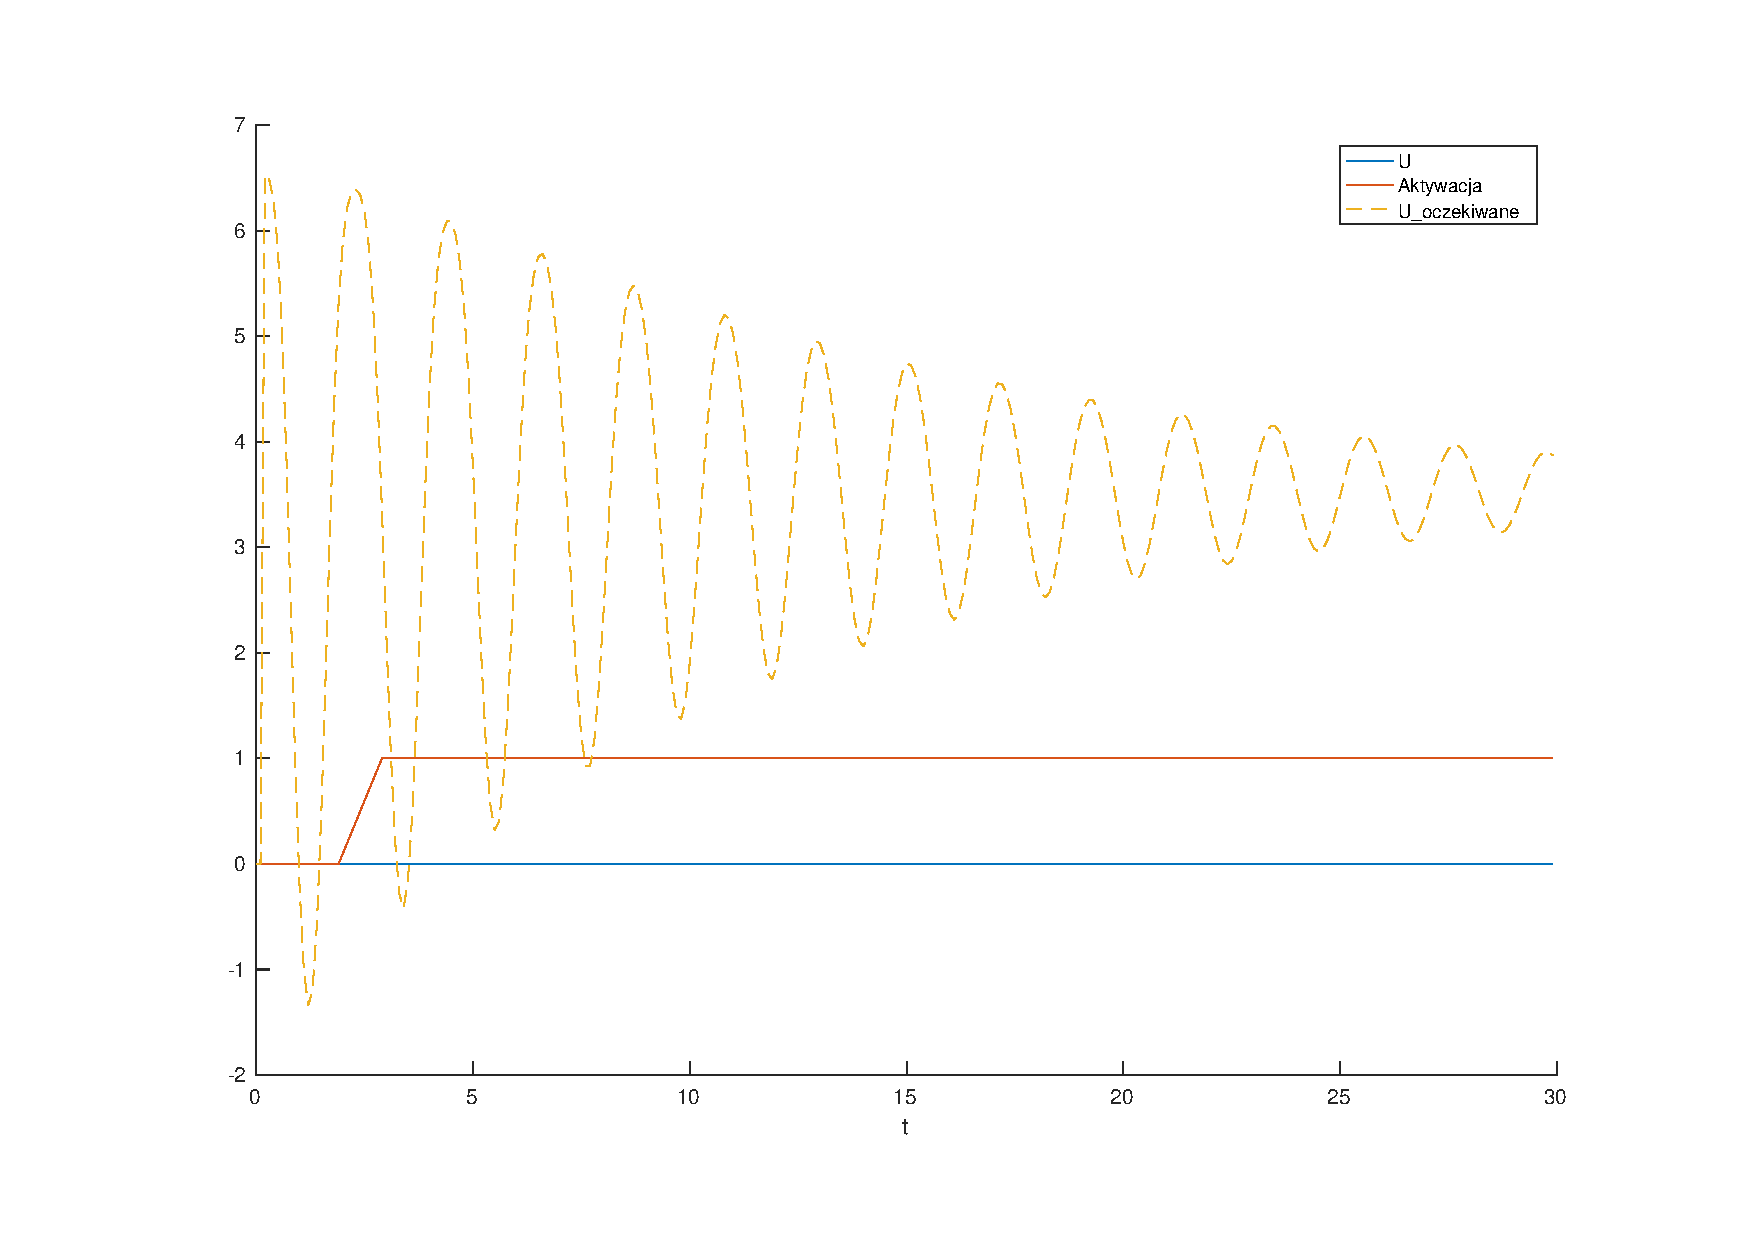
\includegraphics[width=\linewidth]{test_u}
		\caption{Sterowanie (U). Przerywana linia prezentuje sterowanie potrzebne w celu kompensacji grawitacji.}
		\label{fig:system_u}
	\end{subfigure}

	\caption{Symulacja układu z parametrami $T=0.01$, $m = 2$, $r = 1.5$, $k = 16$, $b = 2$. Brak kompensacji grawitacji.}
	\label{fig:system}
\end{figure}


\begin{figure}
	\centering
	\begin{subfigure}{.5\textwidth}
		\centering
		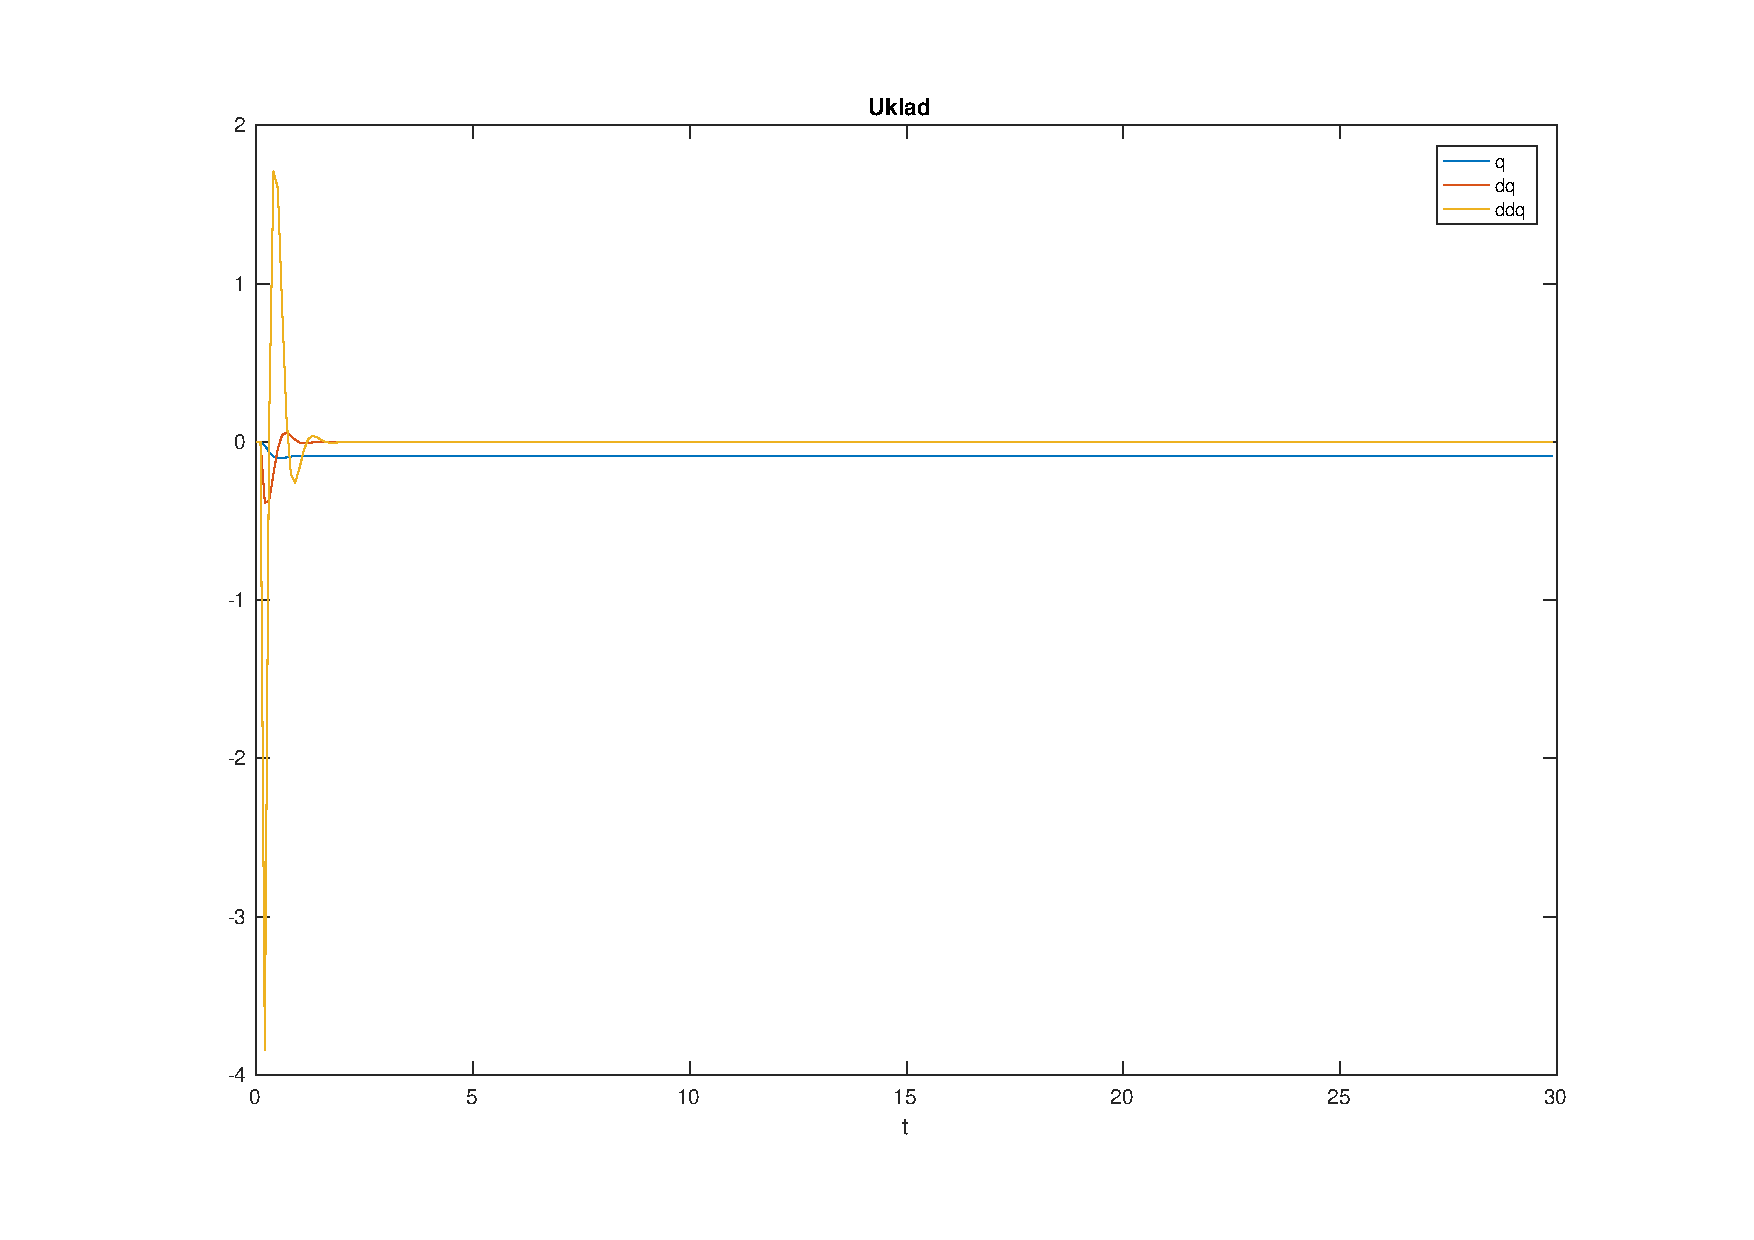
\includegraphics[width=\linewidth]{mala_p}
		\caption{Stan układu. Pozycja (q), prędkość (dq) i przyspieszenie (ddq).}
		\label{fig:mala_p}
	\end{subfigure}%
	\begin{subfigure}{.5\textwidth}
		\centering
		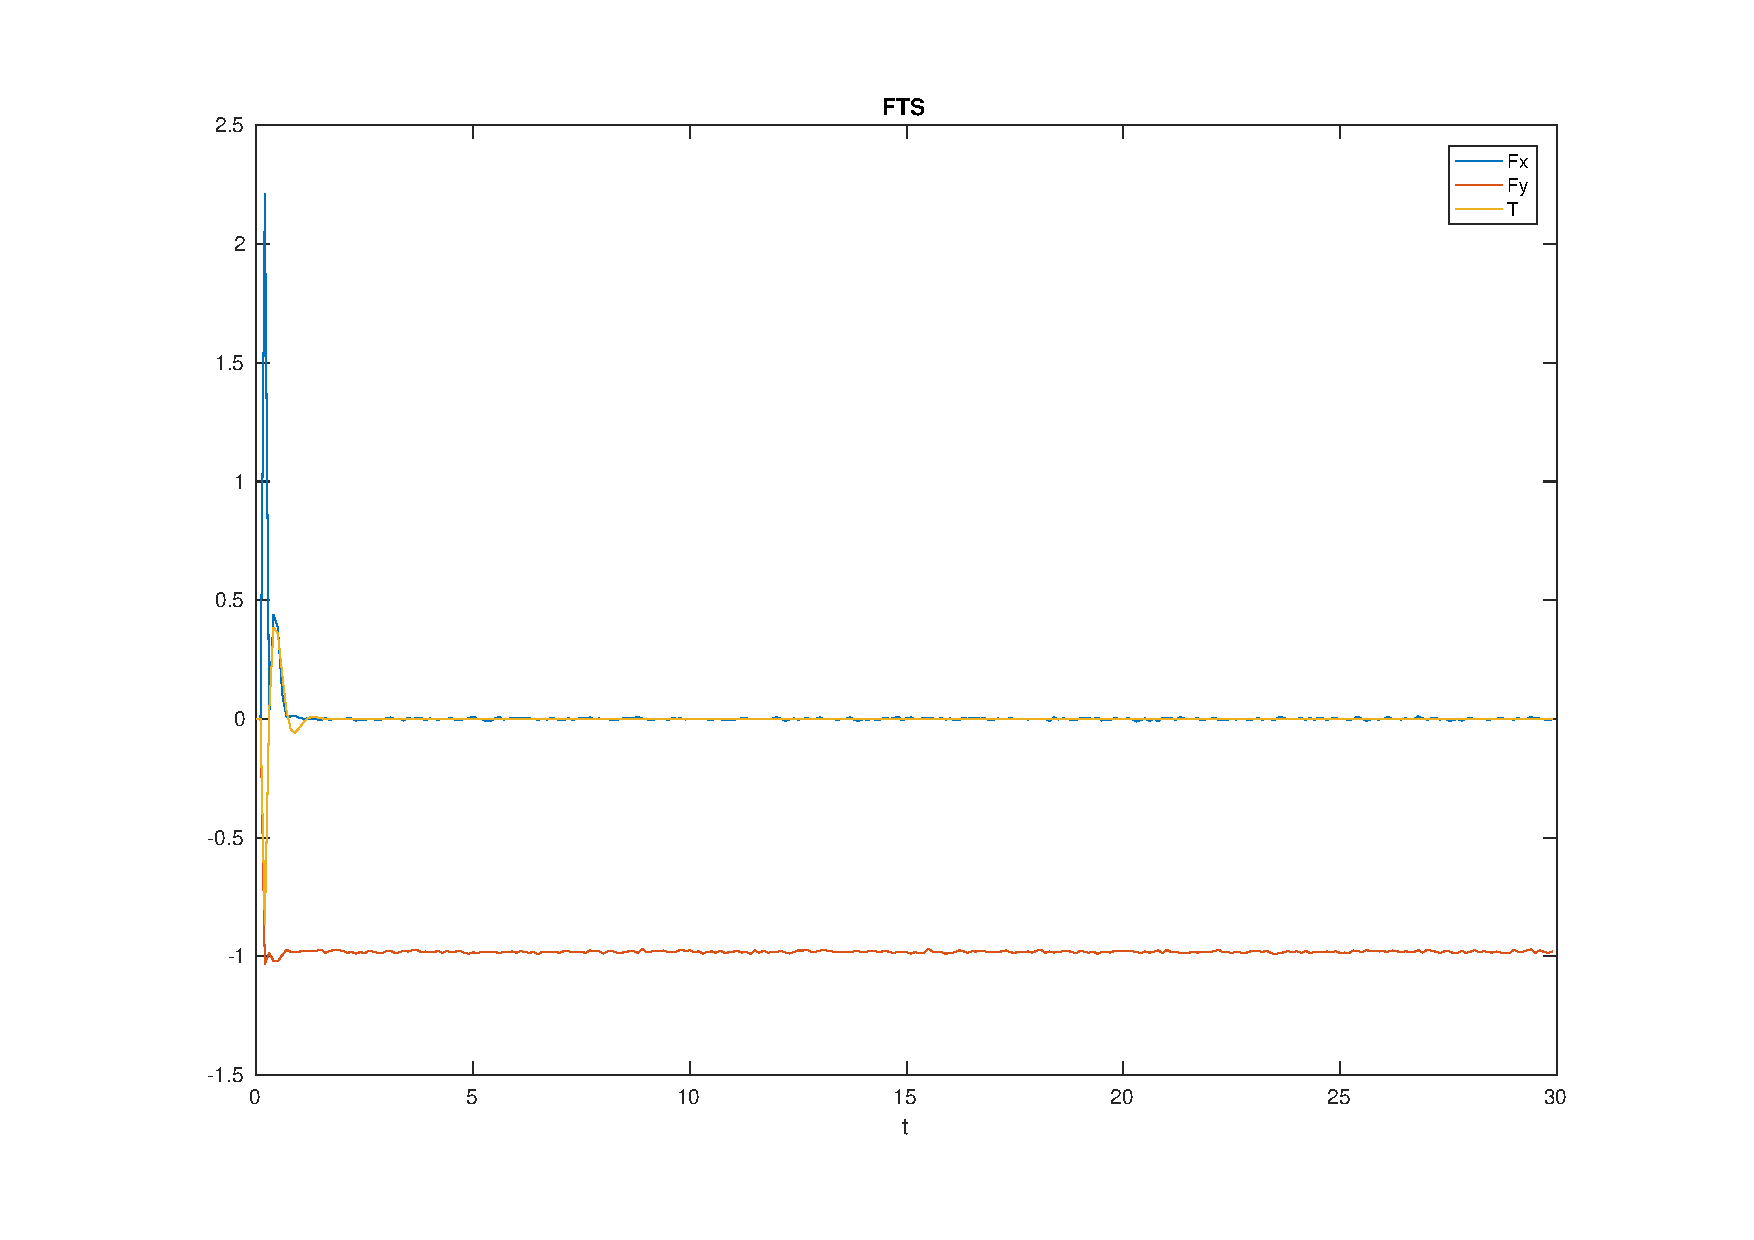
\includegraphics[width=\linewidth]{mala_s}
		\caption{Odczyty czujnika FTS. Siła odczytana w osi $OX$ (Fx), w osi $OY$ (Fy) oraz moment siły (T).}
		\label{fig:mala_s}
	\end{subfigure}
	\begin{subfigure}{.5\textwidth}
		\centering
		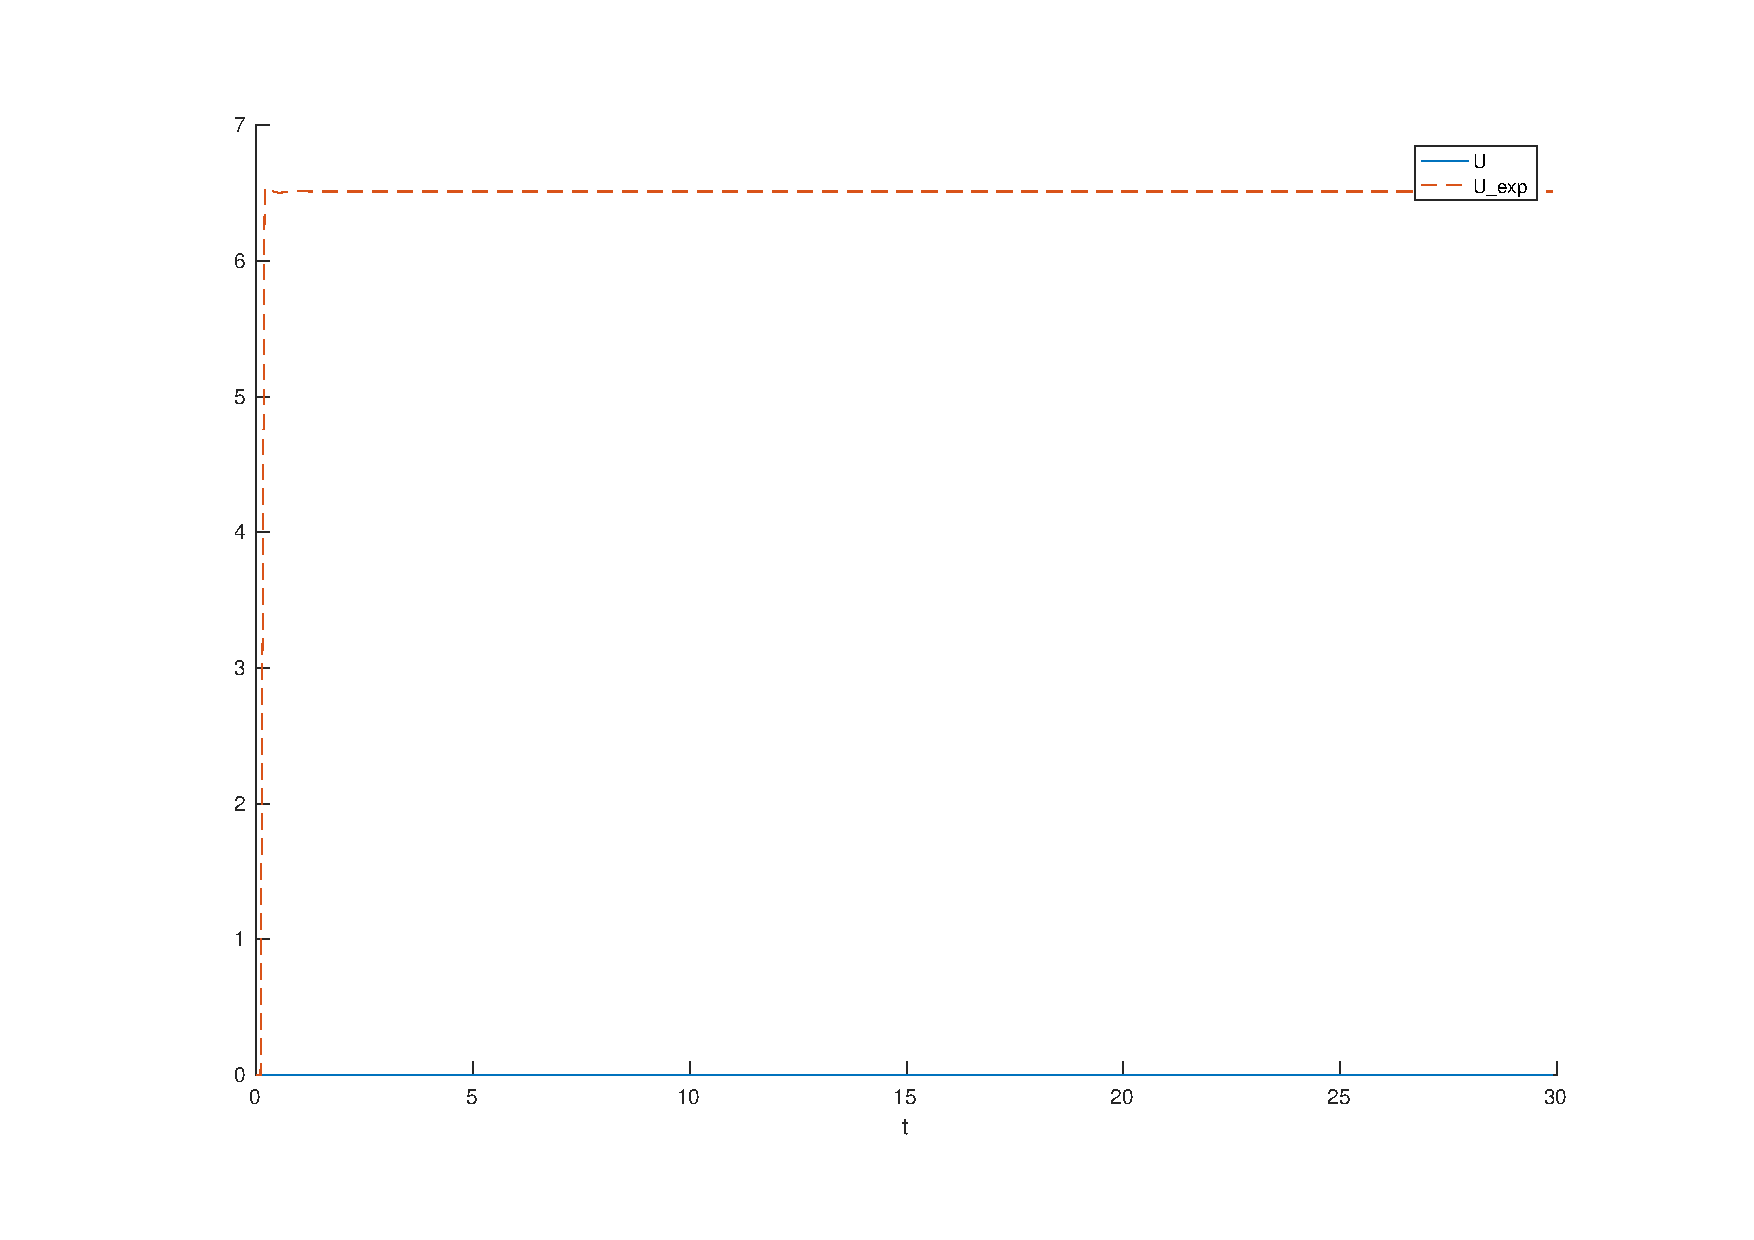
\includegraphics[width=\linewidth]{mala_u}
		\caption{Sterowanie (U). Przerywana linia prezentuje sterowanie potrzebne w celu kompensacji grawitacji.}
		\label{fig:mala_u}
	\end{subfigure}
	\caption{Symulacja układu z parametrami $T=0.01$, $m = 0.1$, $r = 1.5$, $k = 16$, $b = 2$. Brak kompensacji grawitacji.}
	\label{fig:mala}
\end{figure}

\begin{figure}
	\centering
	\begin{subfigure}{.5\textwidth}
		\centering
		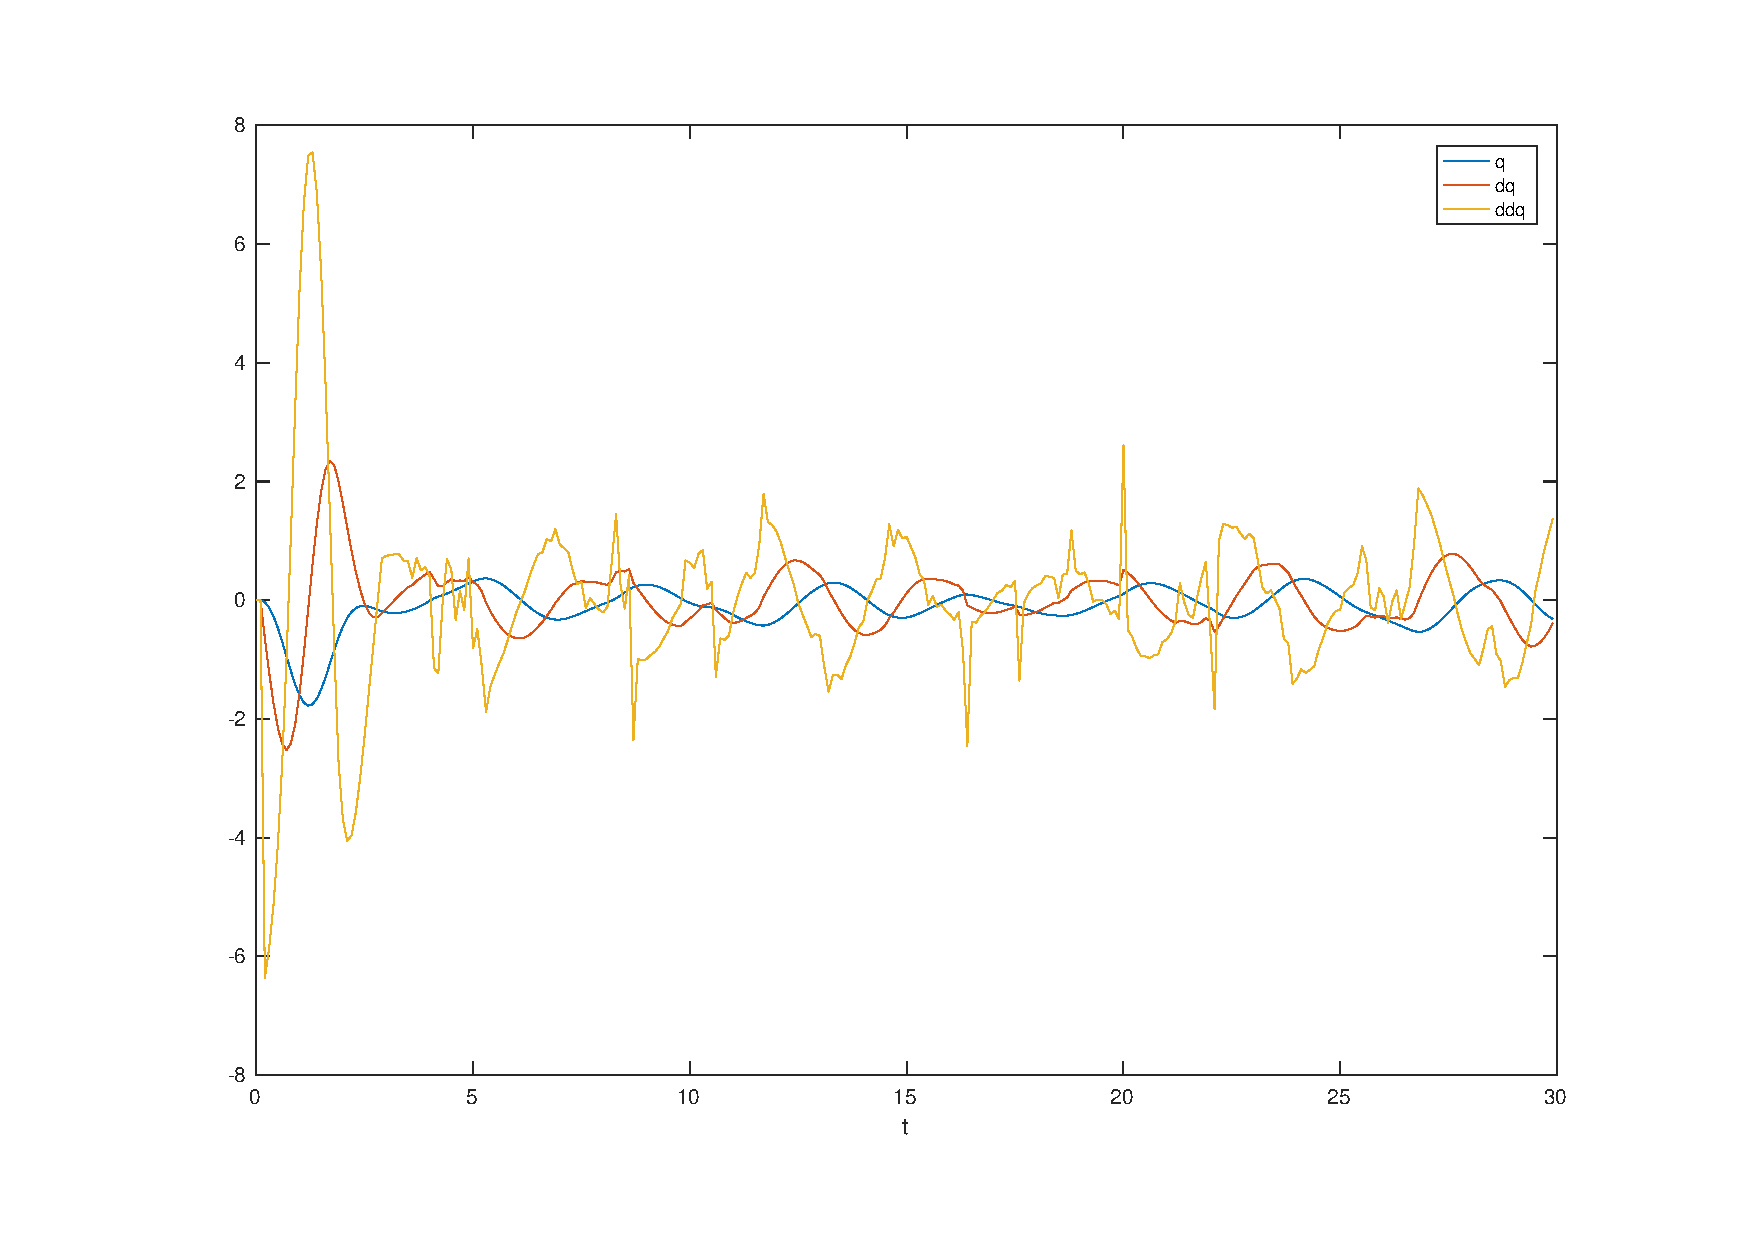
\includegraphics[width=\linewidth]{kompensacja_p}
		\caption{Stan układu. Pozycja (q), prędkość (dq) i przyspieszenie (ddq).}
		\label{fig:kompensacja_p}
	\end{subfigure}%
	\begin{subfigure}{.5\textwidth}
		\centering
		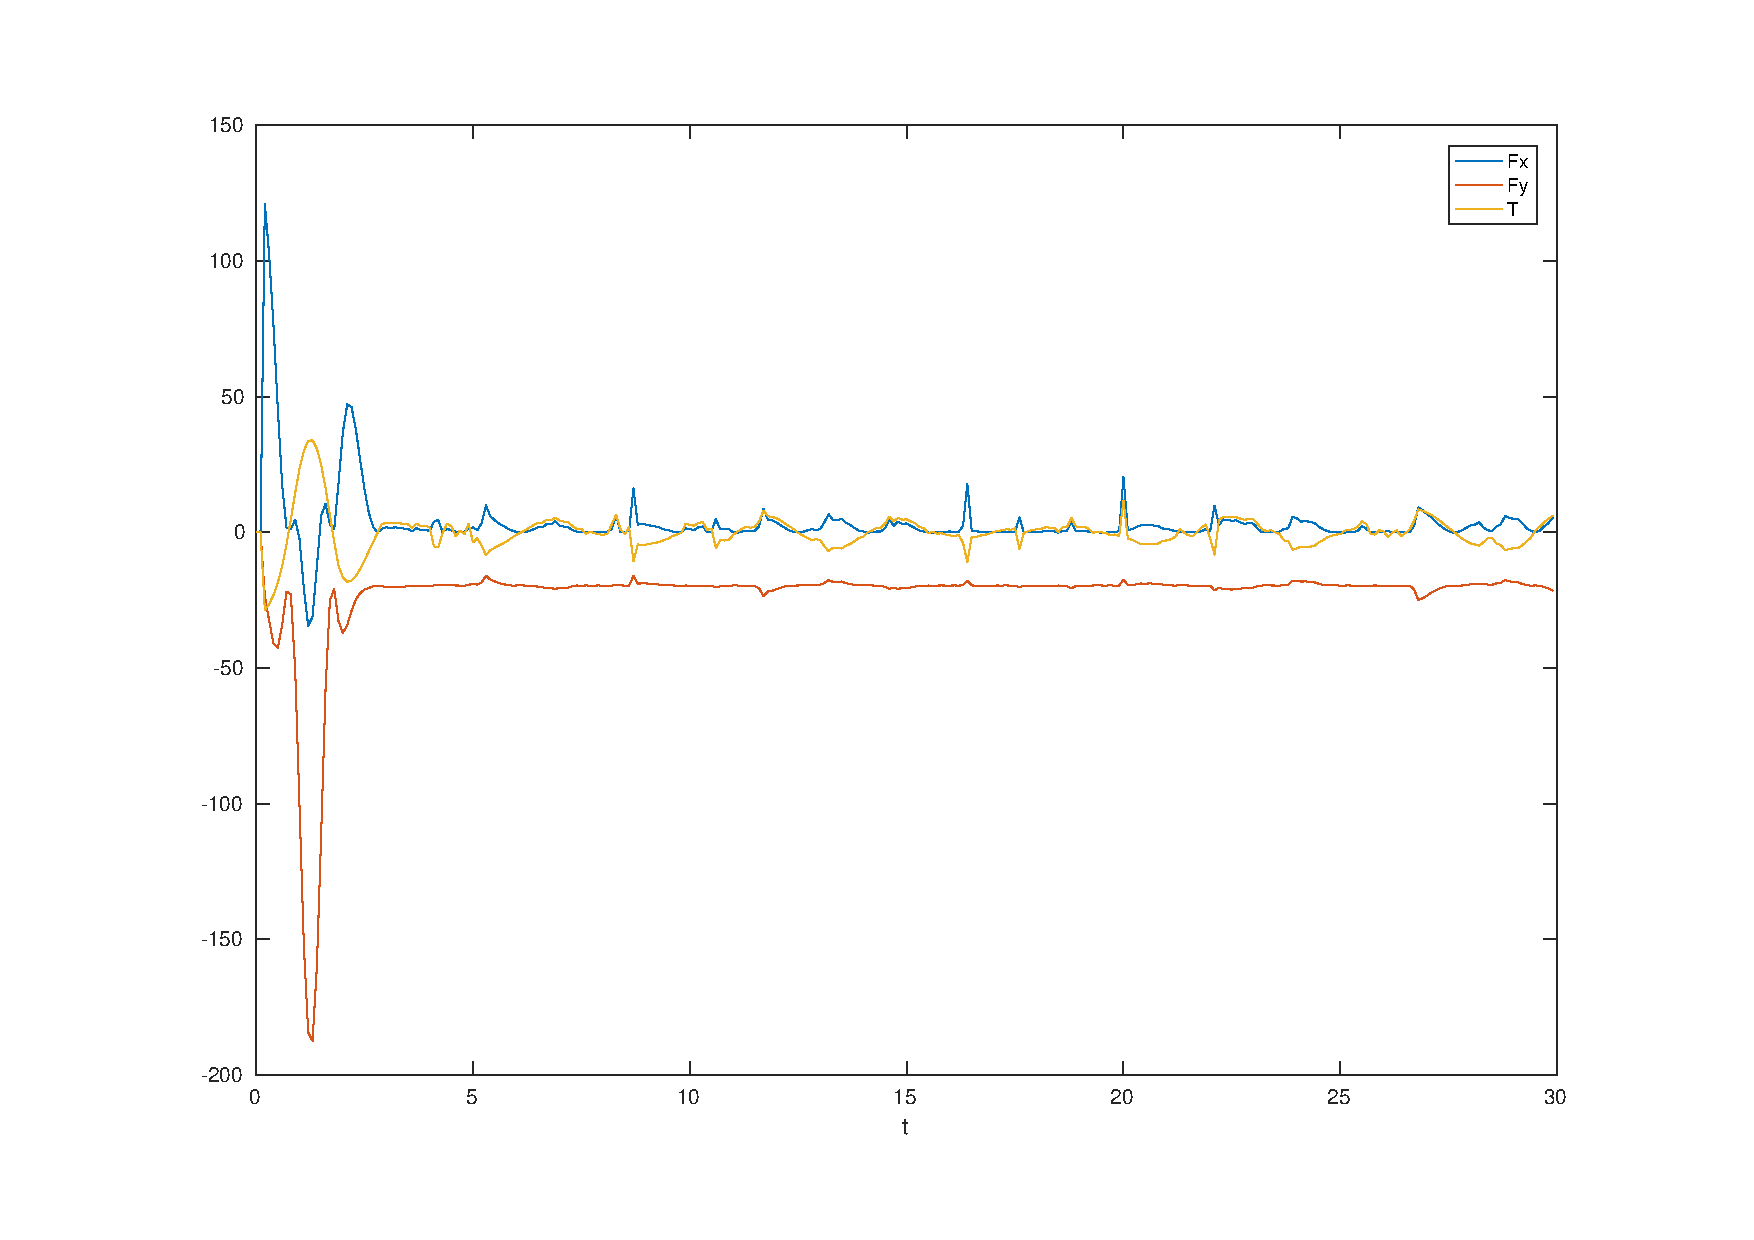
\includegraphics[width=\linewidth]{kompensacja_s}
		\caption{Odczyty czujnika FTS. Siła odczytana w osi $OX$ (Fx), w osi $OY$ (Fy) oraz moment siły (T).}
		\label{fig:kompensacja_s}
	\end{subfigure}
	\begin{subfigure}{.5\textwidth}
		\centering
		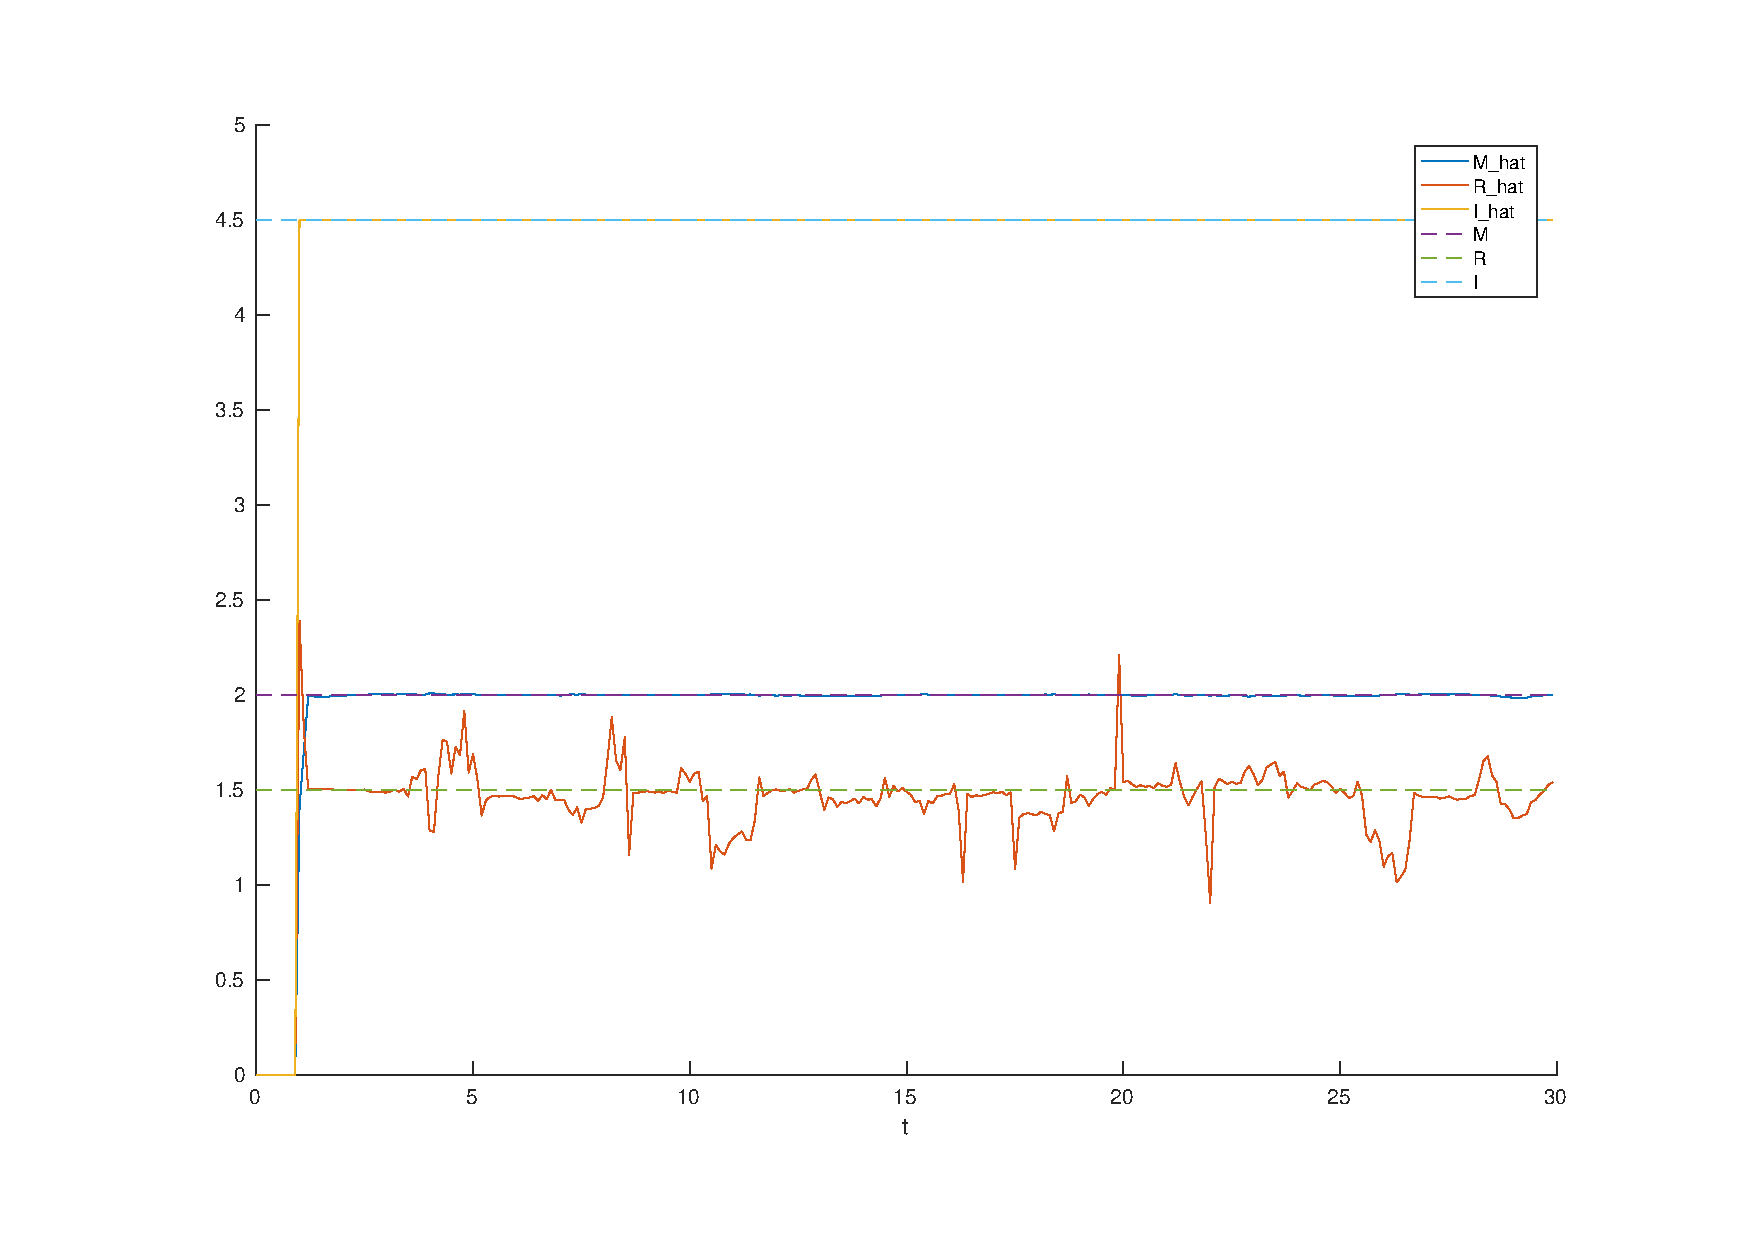
\includegraphics[width=\linewidth]{kompensacja_c}
		\caption{Estymacja parametrów z czujnika sił. Masa (M\_hat), promień (R\_hat) i inercja (I\_hat). Przerywane linie pokazują rzeczywiste wartości parametrów.}
		\label{fig:kompensacja_c}
	\end{subfigure}%
	\begin{subfigure}{.5\textwidth}
		\centering
		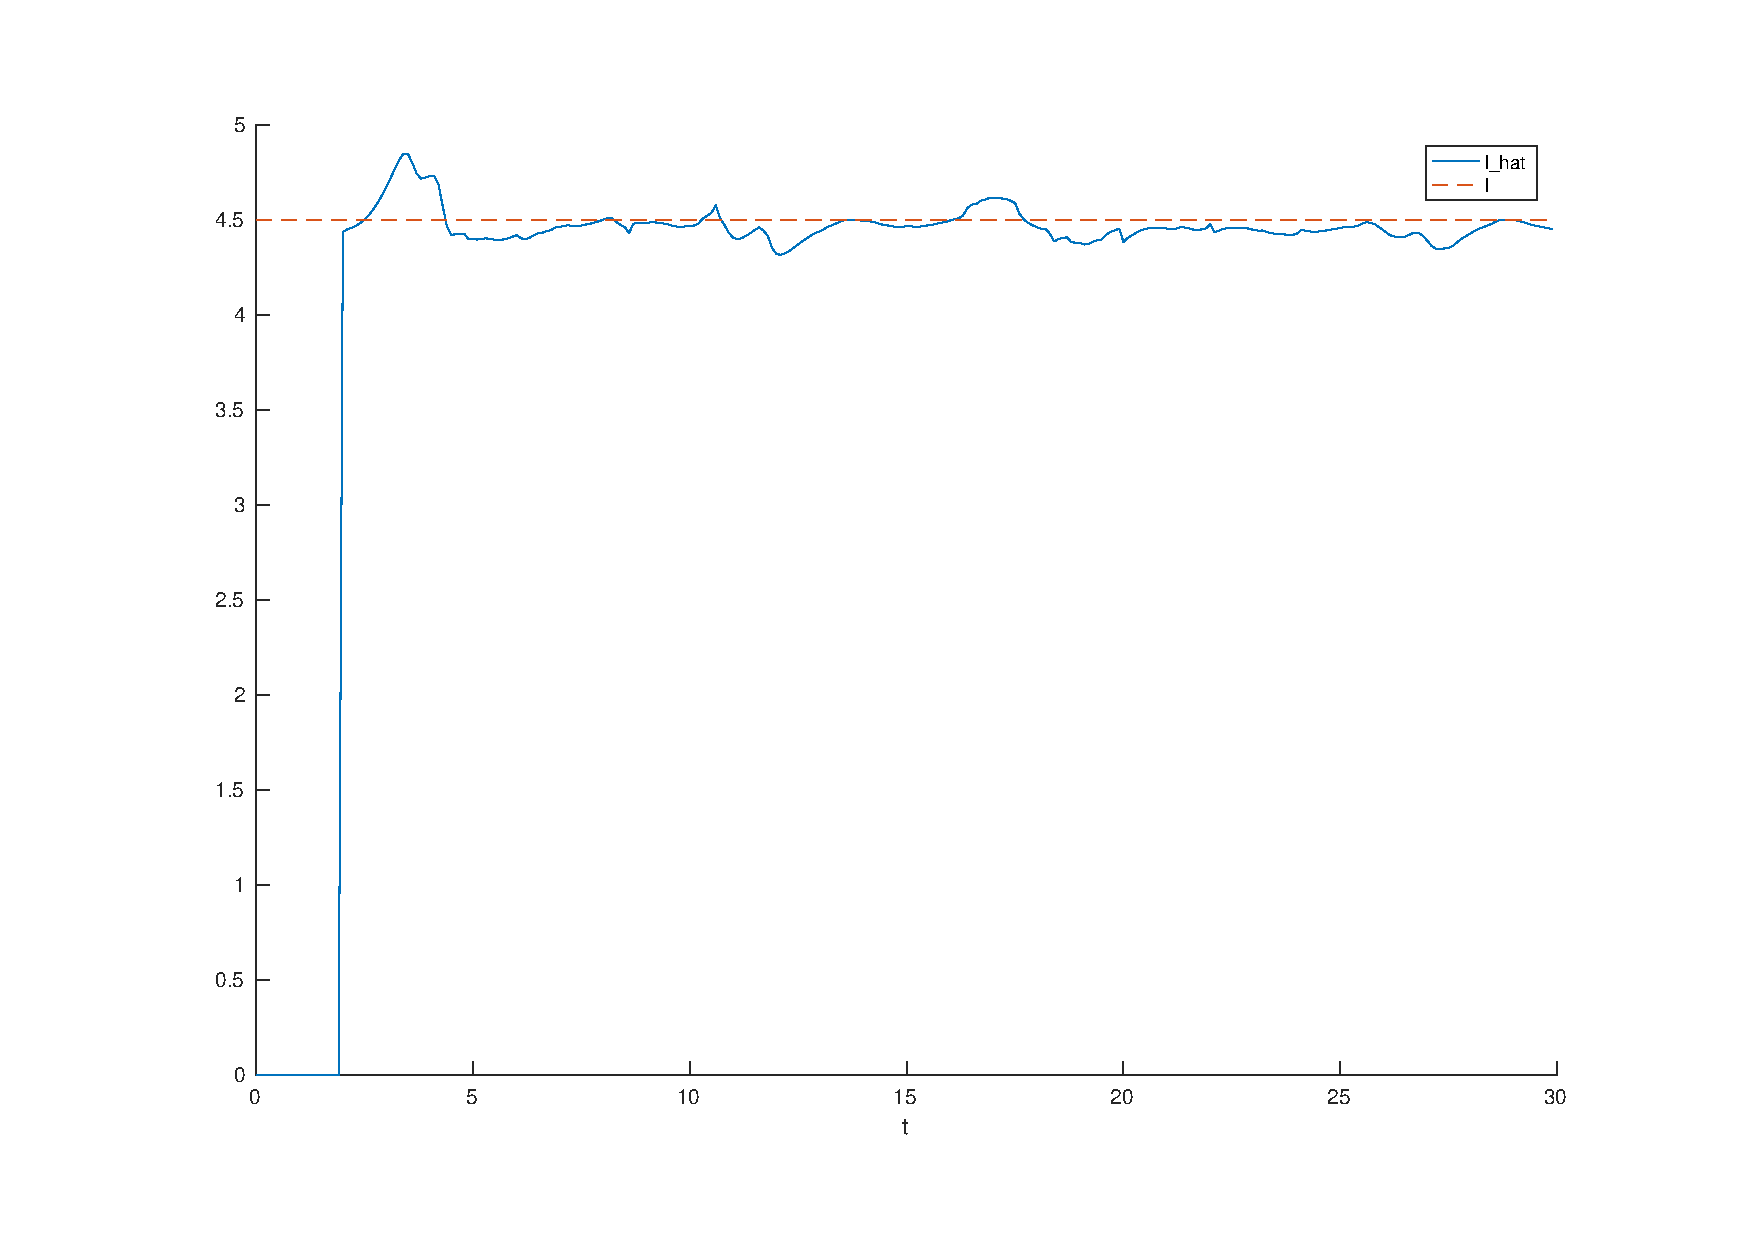
\includegraphics[width=\linewidth]{kompensacja_r}
		\caption{Estymacja inercji (I\_hat) z równań stanu. Przerywana linia pokazuje rzeczywiste wartości parametru.}
		\label{fig:kompensacja_r}
	\end{subfigure}

	\begin{subfigure}{.5\textwidth}
		\centering
		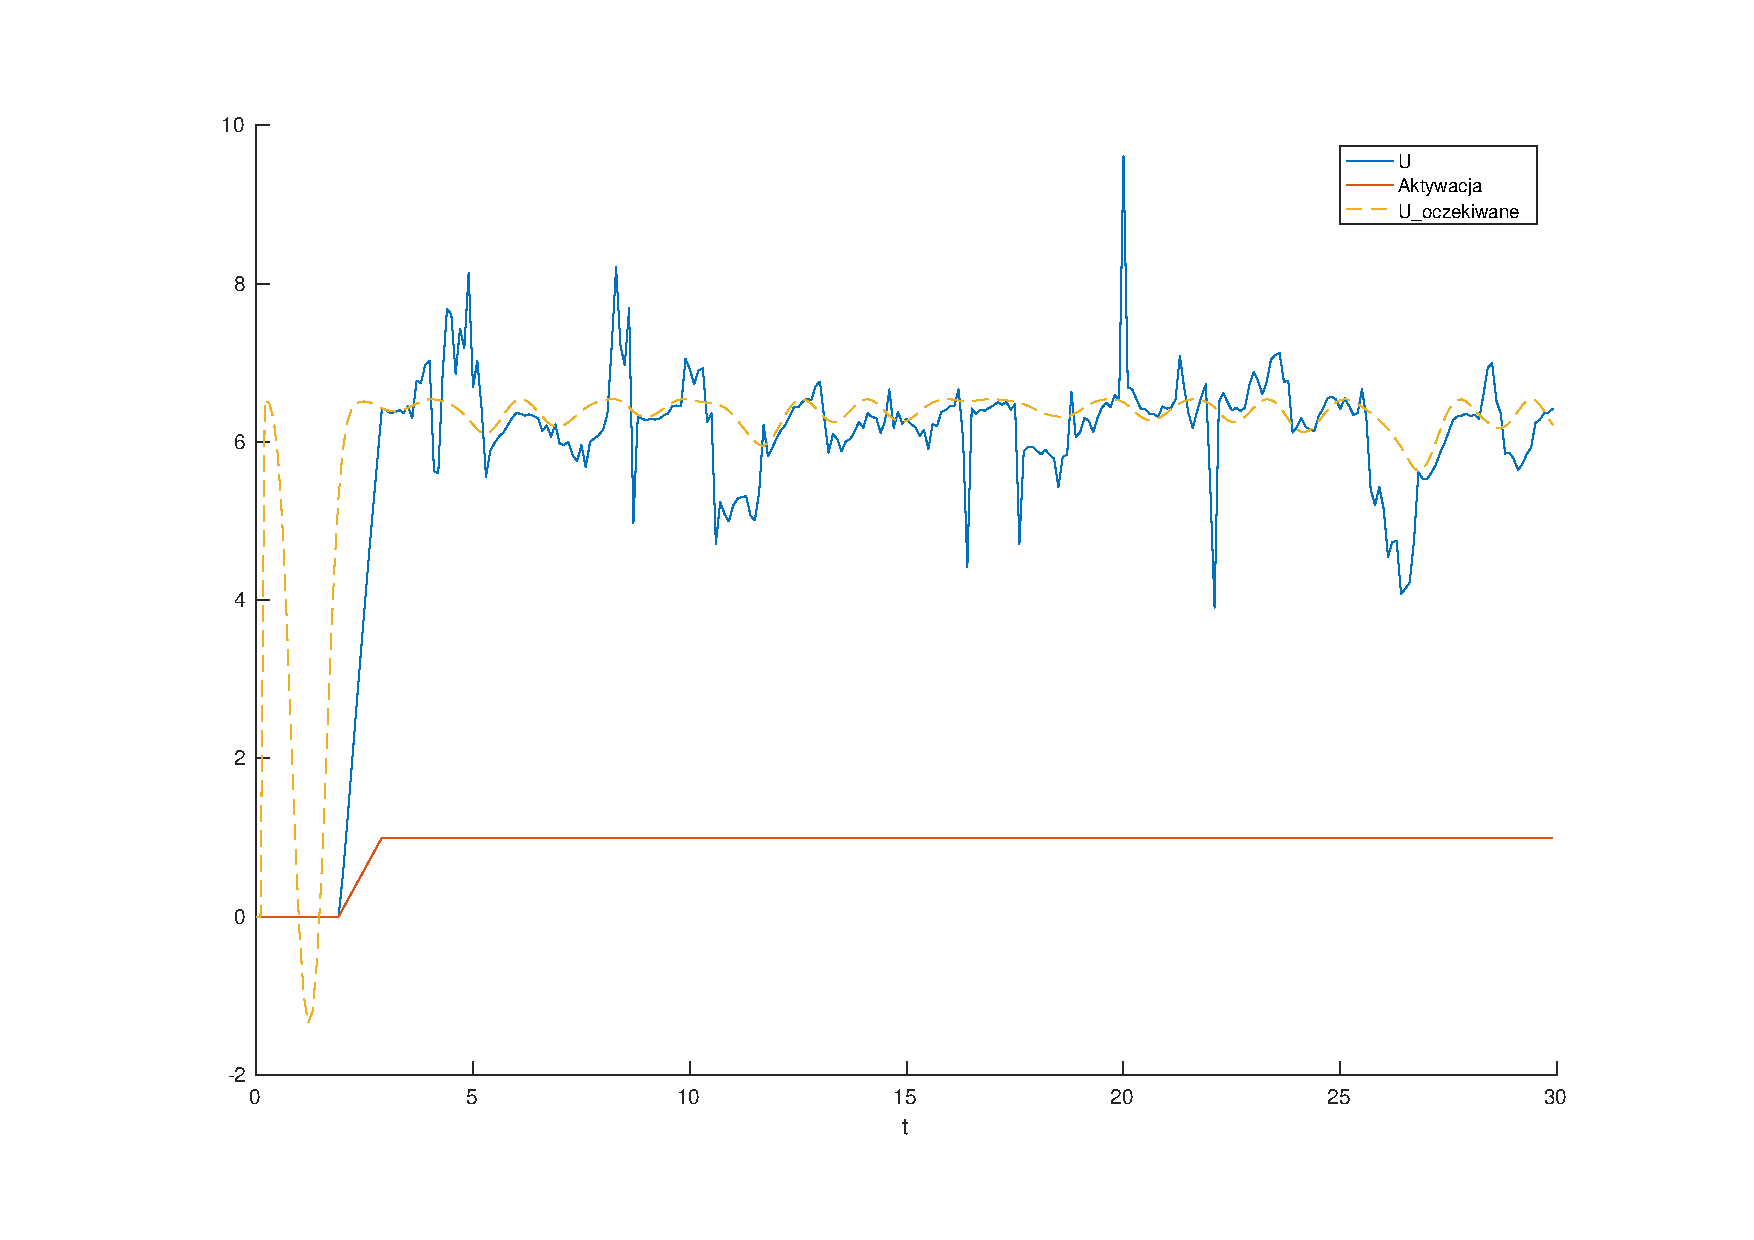
\includegraphics[width=\linewidth]{kompensacja_u}
		\caption{Sterowanie (U). Przerywana linia prezentuje sterowanie potrzebne w celu kompensacji grawitacji. Zaprezentowano funkcję aktywacji momentu kompensacji grawitacji.}
		\label{fig:kompensacja_u}
	\end{subfigure}

	\caption{Symulacja układu z parametrami $T=0.01$, $m = 2$, $r = 1.5$, $k = 16$, $b = 2$. Załączona kompensacja grawitacji. Parametry potrzebne do estymacji uzyskane z FTS.}
	\label{fig:kompensacja}
\end{figure}

\begin{figure}
	\centering
	\begin{subfigure}{.5\textwidth}
		\centering
		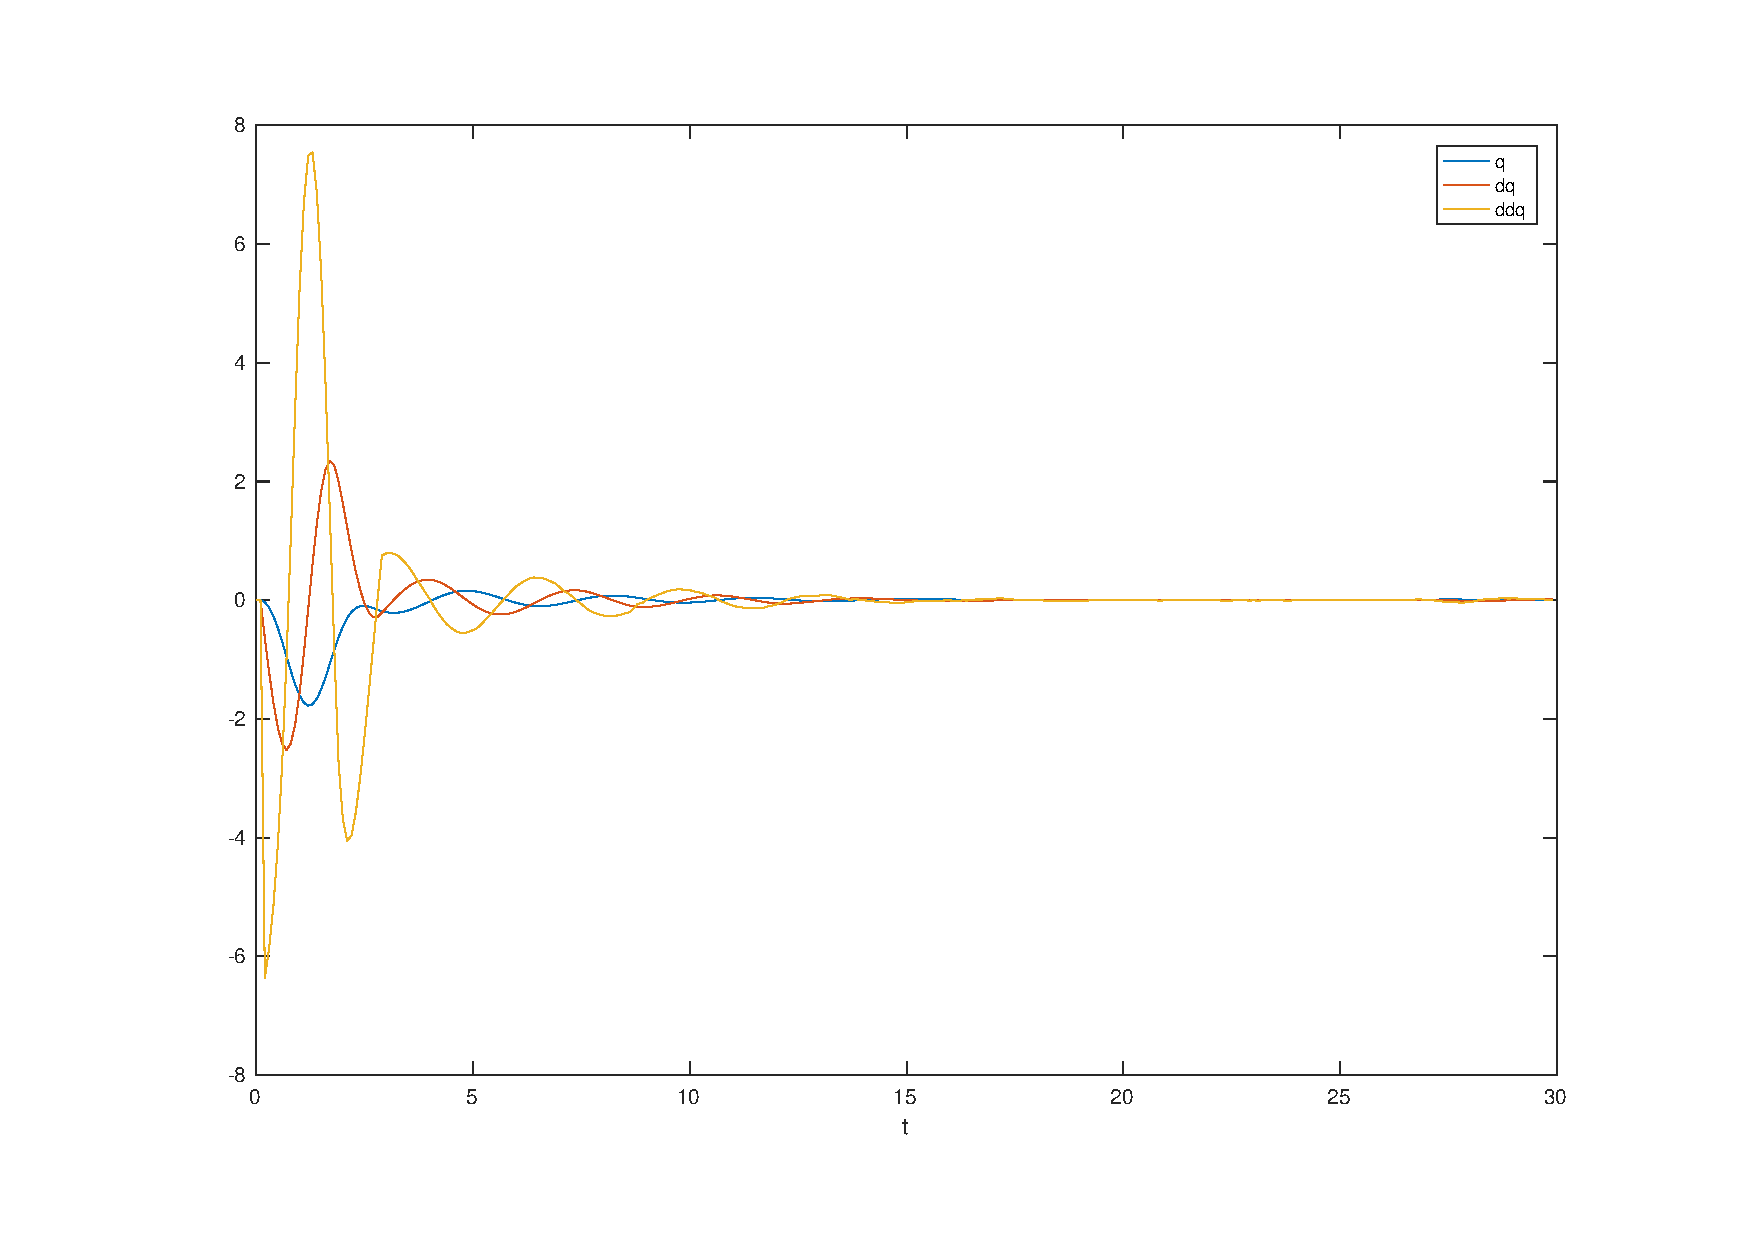
\includegraphics[width=\linewidth]{mrozenie_p}
		\caption{Stan układu. Pozycja (q), prędkość (dq) i przyspieszenie (ddq).}
		\label{fig:mrozenie_p}
	\end{subfigure}%
	\begin{subfigure}{.5\textwidth}
		\centering
		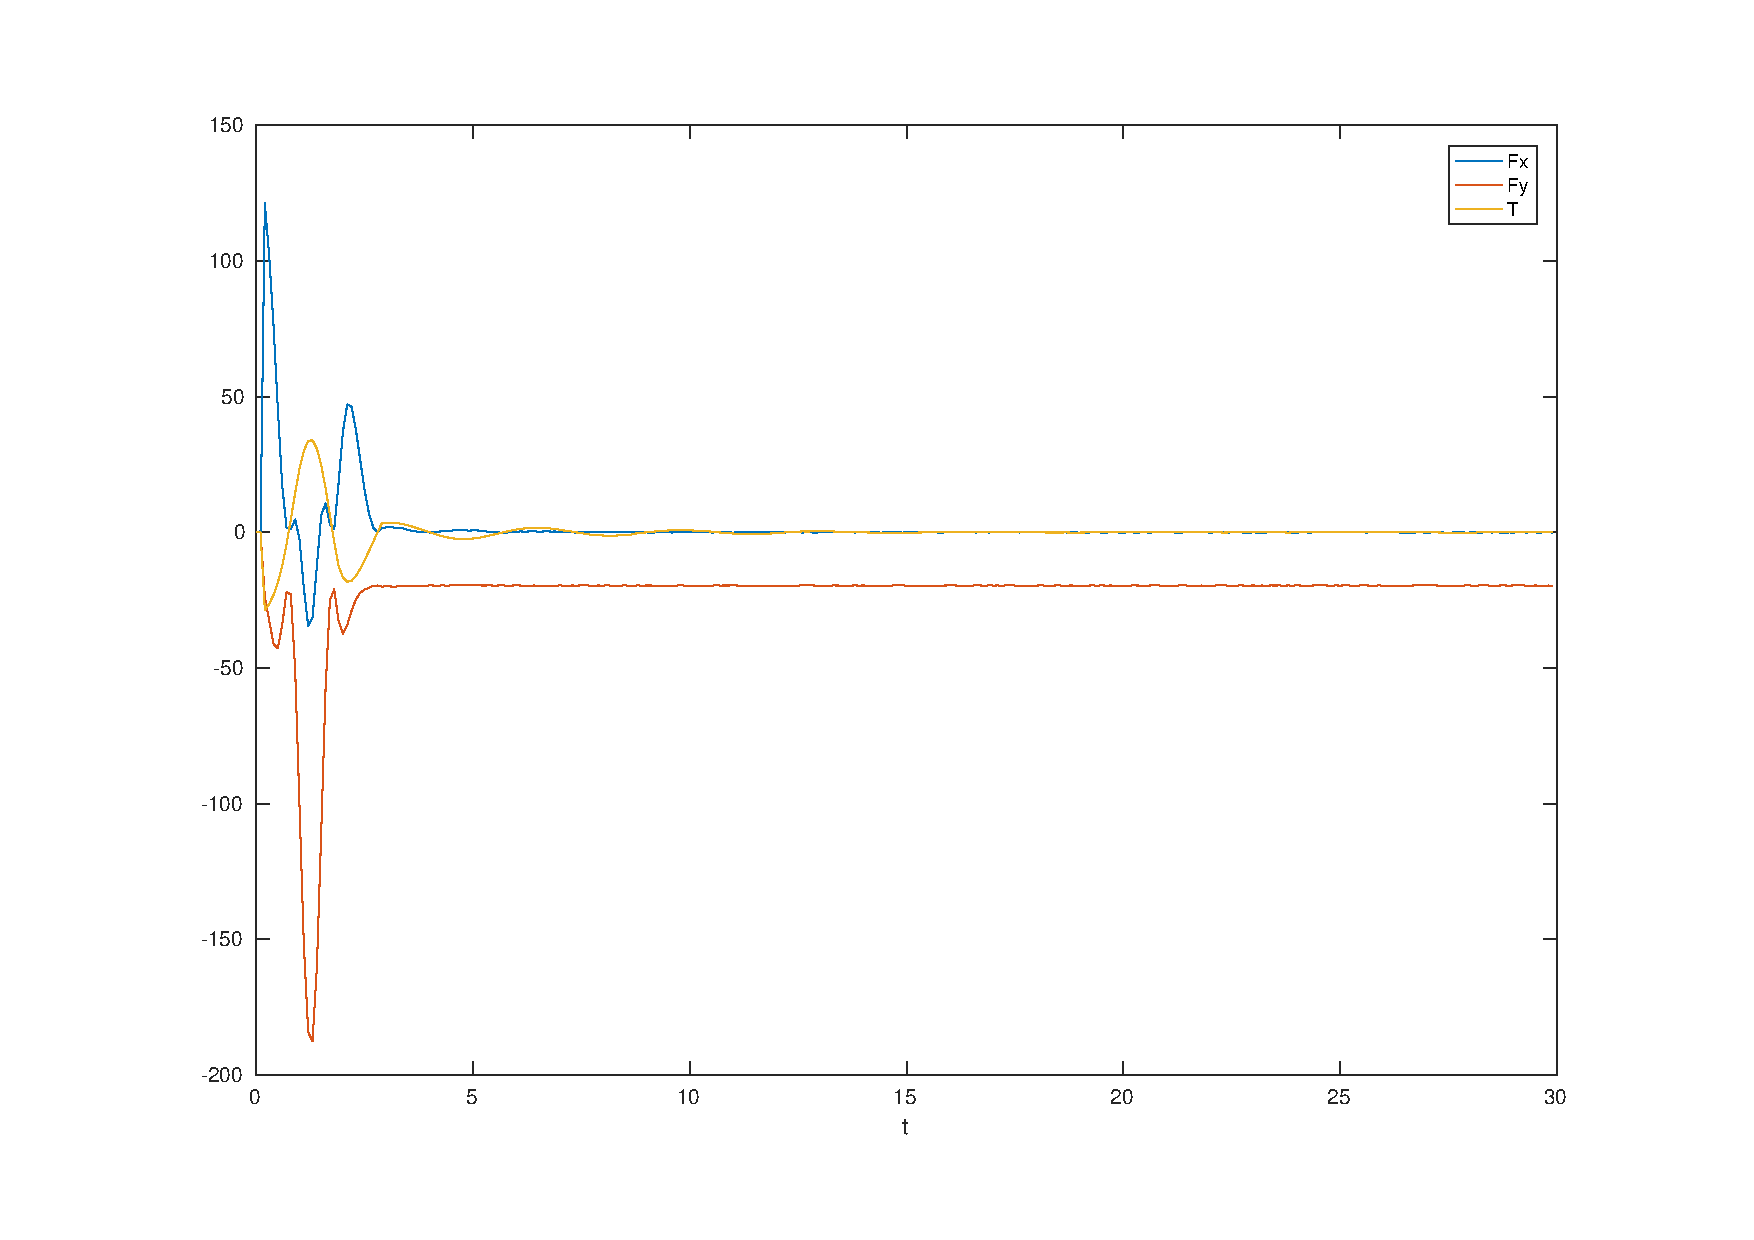
\includegraphics[width=\linewidth]{mrozenie_s}
		\caption{Odczyty czujnika FTS. Siła odczytana w osi $OX$ (Fx), w osi $OY$ (Fy) oraz moment siły (T).}
		\label{fig:mrozenie_s}
	\end{subfigure}
	\begin{subfigure}{.5\textwidth}
		\centering
		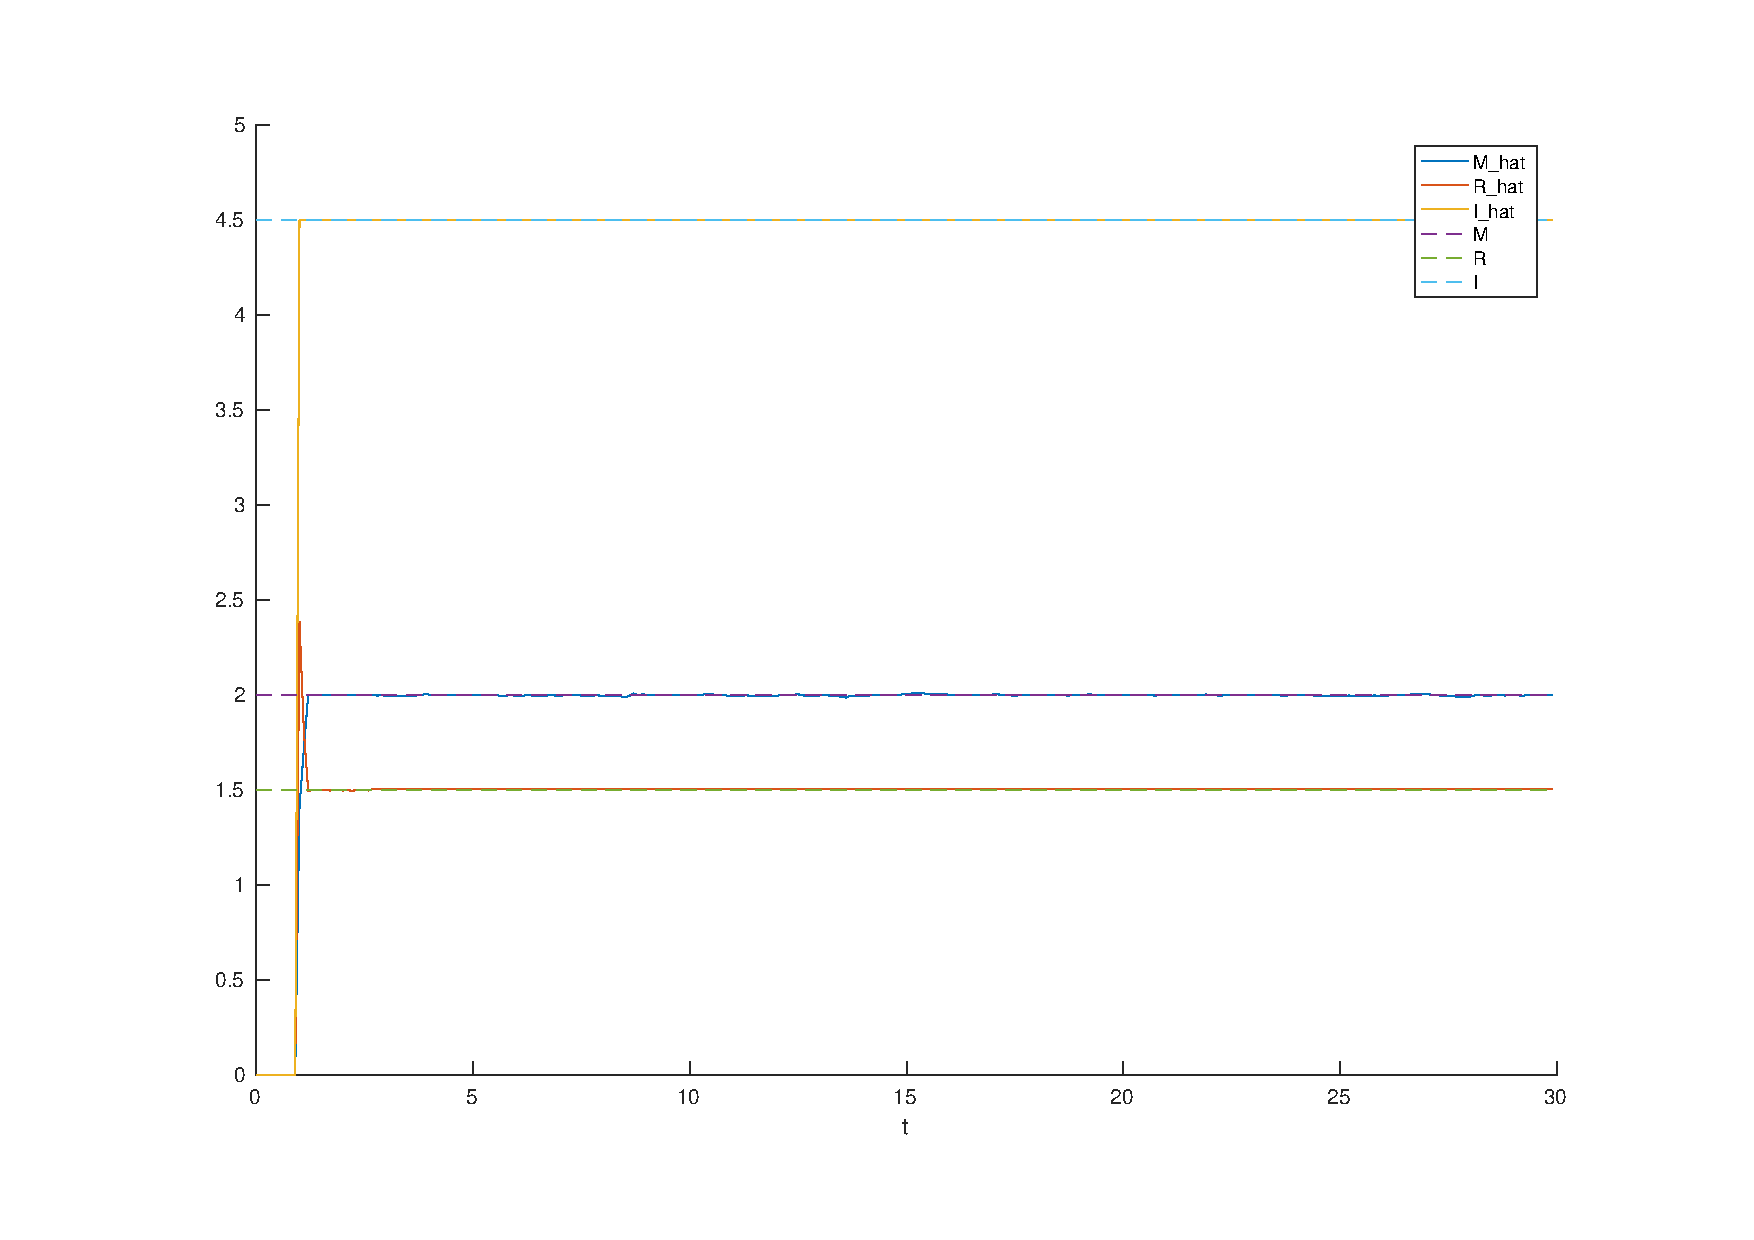
\includegraphics[width=\linewidth]{mrozenie_c}
		\caption{Estymacja parametrów z czujnika sił. Masa (M\_hat), promień (R\_hat) i inercja (I\_hat). Przerywane linie pokazują rzeczywiste wartości parametrów.}
		\label{fig:mrozenie_c}
	\end{subfigure}%
	\begin{subfigure}{.5\textwidth}
		\centering
		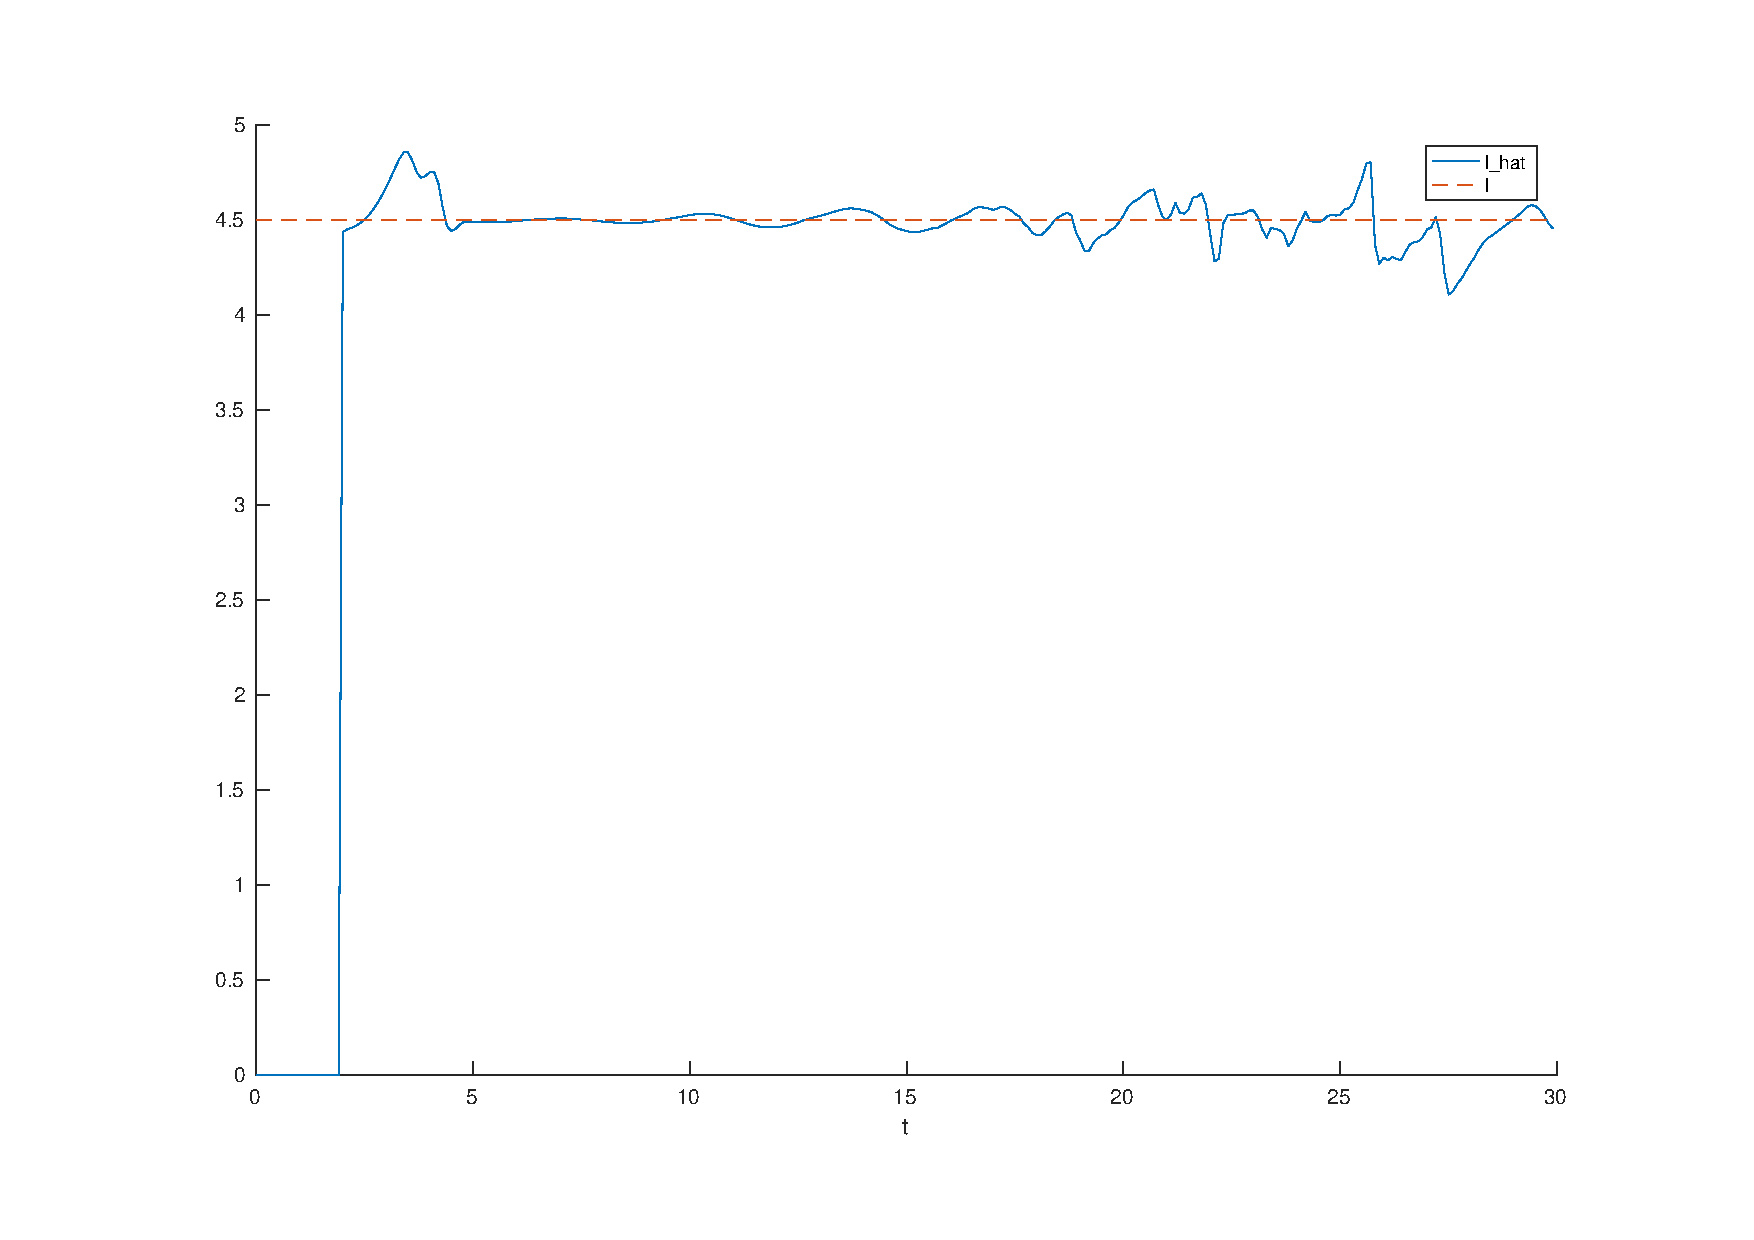
\includegraphics[width=\linewidth]{mrozenie_r}
		\caption{Estymacja inercji (I\_hat) z równań stanu. Przerywana linia pokazuje rzeczywiste wartości parametru.}
		\label{fig:mrozenie_r}
	\end{subfigure}

	\begin{subfigure}{.5\textwidth}
		\centering
		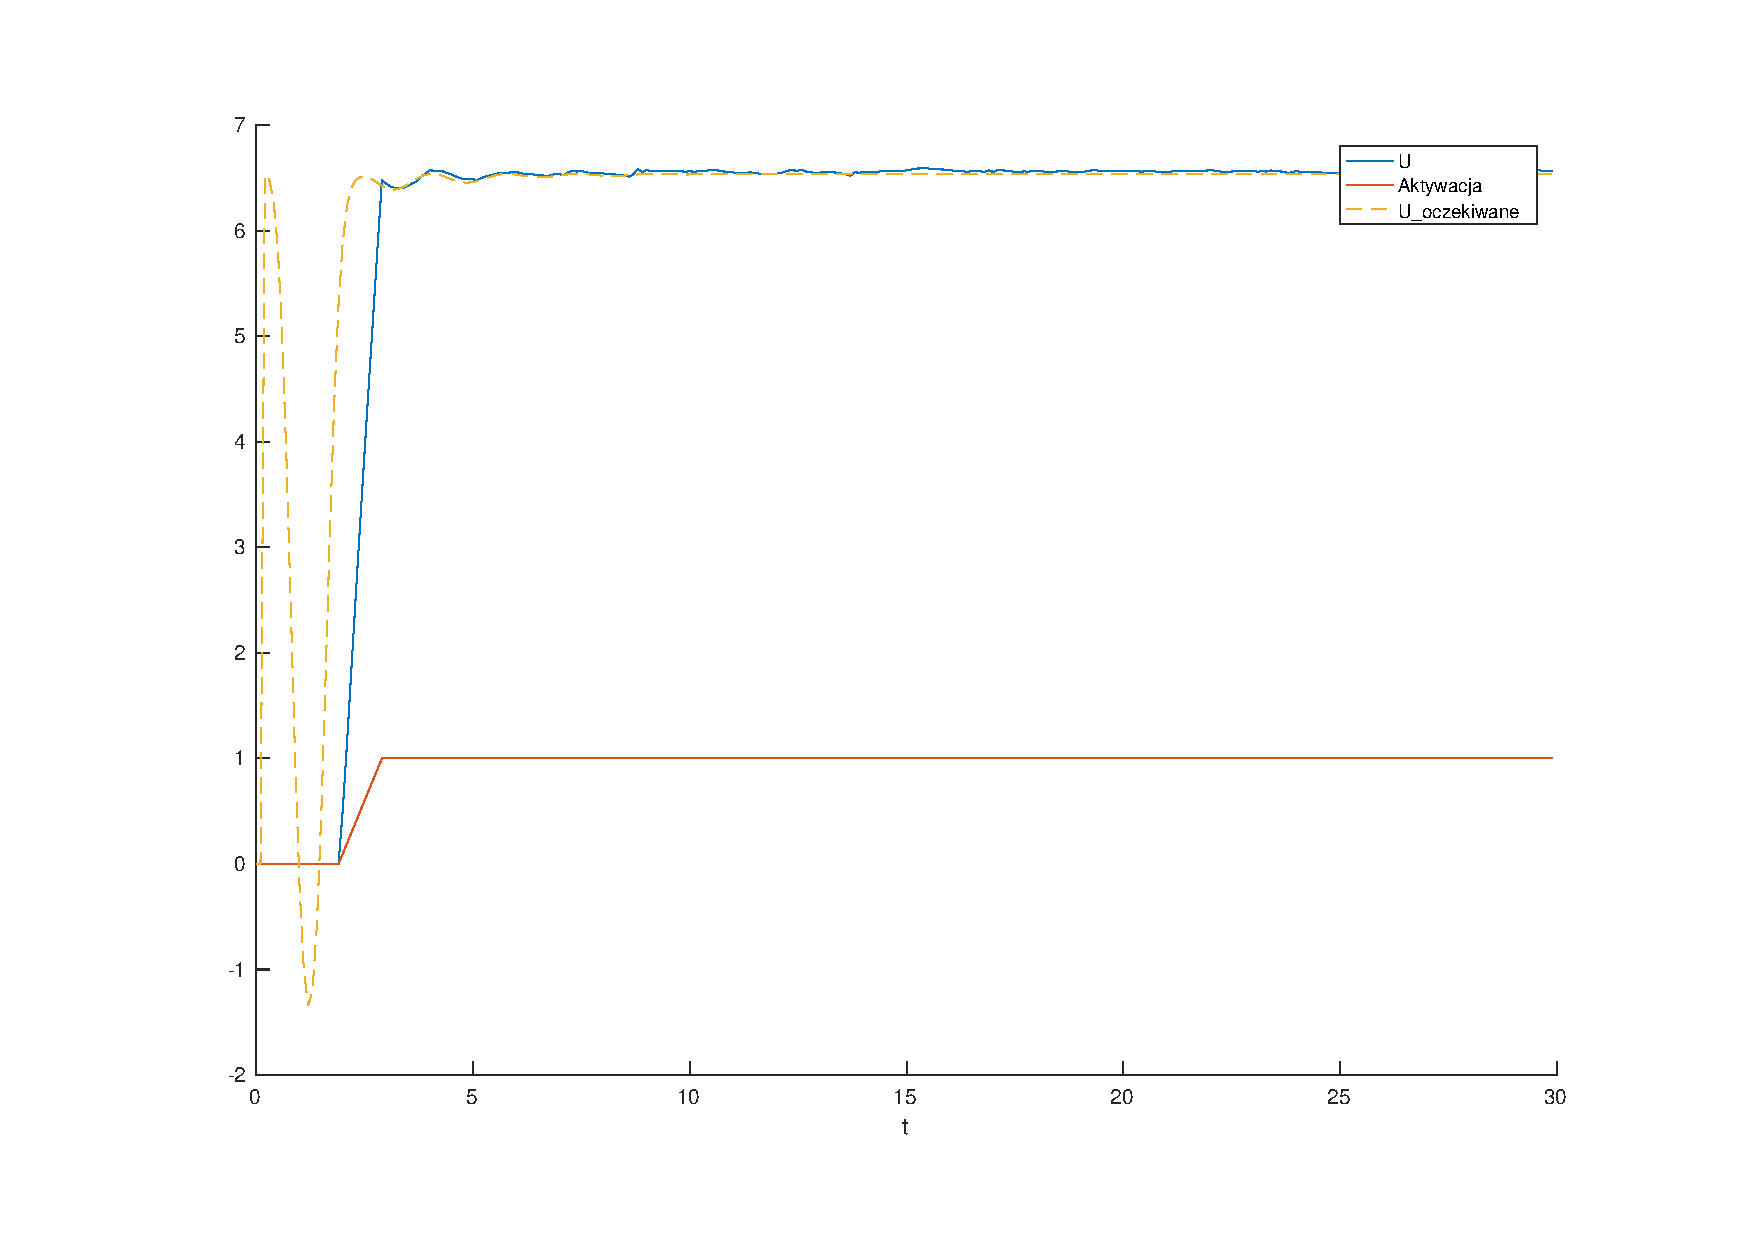
\includegraphics[width=\linewidth]{mrozenie_u}
		\caption{Sterowanie (U). Przerywana linia prezentuje sterowanie potrzebne w celu kompensacji grawitacji. Zaprezentowano funkcję aktywacji momentu kompensacji grawitacji.}
		\label{fig:mrozenie_u}
	\end{subfigure}

	\caption{Symulacja układu z parametrami $T=0.01$, $m = 2$, $r = 1.5$, $k = 16$, $b = 2$. Załączona kompensacja grawitacji. Po pierwszych 2 sekundach symulacji zamrożono estymację parametru $r$. Parametry potrzebne do estymacji uzyskane z FTS.}
	\label{fig:mrozenie}
\end{figure}

\end{document}